%%%%%%%%%%%%%%%%%%%%%%%%%%%%%%%%%%%%%%%%%%%%%%%%%%%%%%%%
%
%  FINAL REPORT - Robot Mower
% 
%%%%%%%%%%%%%%%%%%%%%%%%%%%%%%%%%%%%%%%%%%%%%%%%%%%%%%%%
\documentclass[final]{cmpreport_02}


% Some package I am using. You may not need them
%
\usepackage{rotating}
\usepackage{subfig}
\usepackage{todonotes}
\usepackage{color}
\usepackage{pdfpages}
\usepackage{cleveref}
\usepackage{natbib}
\usepackage{float}
\usepackage{hyperref}
\usepackage{algorithm}
\usepackage{algorithmicx}
\usepackage{algpseudocode}



%\setkeys{Gin}{draft}

%%%%%%%%%%%%%%%%%%%%%%%%%%%%%%%%%%%%%%%%%%%%%%%%%%%%%%%%
%
%  Fill in the fields with:
%
%  your project title
%  your name
%  your registration number
%  your supervisor's name
%
%%%%%%%%%%%%%%%%%%%%%%%%%%%%%%%%%%%%%%%%%%%%%%%%%%%%%%%%
\title{Robot Mower Mapping and Pathing}
%%%%%%%%%%%%%%%%%%%%%%%%%%%%%%%%%%%%%%%%%%%%%%%%%%%%%%%%
%
% The author's name is ignored if the following command 
% is not present in the document
%
% Before submitting a PDF of your final report to the 
% project database you may comment out the command
% if you are worried about lack of anonimity.
%
%%%%%%%%%%%%%%%%%%%%%%%%%%%%%%%%%%%%%%%%%%%%%%%%%%%%%%%%
\author{Toby William Towler}

\registration{100395626}
\supervisor{Edwin Ren}

%%%%%%%%%%%%%%%%%%%%%%%%%%%%%%%%%%%%%%%%%%%%%%%%%%%%%%%%
%
% Fill in the field with your module code.
% this should be:
%
% for BIS project module   -> CMP-6012Y
% for CS project module    -> CMP-6013Y
% for MComp project module -> CMP-7043Y
%
%%%%%%%%%%%%%%%%%%%%%%%%%%%%%%%%%%%%%%%%%%%%%%%%%%%%%%%%
\ccode{CMP-6013Y}

%%%%%%%%%%%%%%%%%%%%%%%%%%%%%%%%%%%%%%%%%%%%%%%%%%%%%%%%
%
% Comment out if confidential report.
% The command should be used if the project is subjected 
% to a Non Disclosure Agreement.
%
% Three examples of the use of the \confidential command. 
% Please ask your supervisor what confidential statement 
% should be used, if appropriate.
%
%%%%%%%%%%%%%%%%%%%%%%%%%%%%%%%%%%%%%%%%%%%%%%%%%%%%%%%%
%\confidential{}

%\confidential{The contents of this report remain confidential for two years and should not be discussed or disclosed to any third party without the prior written permission from the School of Computing Sciences, the University of East Anglia}

%\confidential{The information contained in this document is confidential, privileged and only for the information of the intended recipient and may not be used, published or redistributed without the prior written consent of FruitName Ltd}


\summary{
The "Robot Mower" is a self-contained lawn mower unit aimed at maintaining golf courses. 
This project is a redesign of the movement planning systems, enhancing and automating the map generation and complete coverage path planning techniques through external libraries and machine learning methods.
The complete coverage path planning module adapts a powerful C++ library designed for agricultural use complete with obstacle avoidance, to the golf course use case.
Map generation is now comprised of an orthophoto or drone image input to a custom MaskRCNN PyTorch machine learning model trained on Danish golf courses to ensure consistent and accurate results correctly identifying all classes within this region.
In conclusion, the complete coverage path planning and aerial image map generation successfully automates the route planning issues of the Robot Mower.
\newpage
}

\acknowledgements{
    Edwin Ren, Eden Attlebourgh
}

%%%%%%%%%%%%%%%%%%%%%%%%%%%%%%%%%%%%%%%%%%%%%%%%%%%%%%%%%%%%%%%%%%
%
% If you do want a list of figures and a list of tables
% to appear after the table of contents then comment this line.
% THIS IS NOT ADVISED THOUGH AS IT COUNTS FOR YOUR 40 PAGES!
%
% Note that the class file contains code to avoid
% producing an empty list section (e.g list of figures) if the 
% list is empty (i.e. no figure in document).
%
% The command also prevents inserting a list of figures or tables 
% anywhere else in the document
%
%%%%%%%%%%%%%%%%%%%%%%%%%%%%%%%%%%%%%%%%%%%%%%%%%%%%%%%%%%%%%%%%%%
% \nolist

%%%%%%%%%%%%%%%%%%%%%%%%%%%%%%%%%%%%%%%%%%%%%%%%%%%%%%%%%%%%%%%%%%
%
% Comment out if you want your list of figures and list of
% tables on one page instead of two or more pages, in particular 
% if the lists do not fit on a single page.
%
%%%%%%%%%%%%%%%%%%%%%%%%%%%%%%%%%%%%%%%%%%%%%%%%%%%%%%%%%%%%%%%%%%
% \onePageLists



\begin{document}

\section{Introduction}

\subsection{Robot Mower}
The robot mower is an already existing project developed by previous masters students from the University of East Anglia.

\subsubsection{Physical architecture}
The physical footprint of the mower features a rigid metal frame with a single track at either side for movement.
A central storage compartment houses the bulk of the computational units and a large single battery enabling wireless travel and removing the need for long power cables following the robot around.

Also, there is excess room on top of the unit for additional sensors enabling clearer signals due to the lack of material shielding that comes with being at the highest point of the robot.

A single track running the full length of the robot sits at either side of the chassis enabling full 360° movement and near on the spot turning capabilities.
All large single battery 


\subsubsection{Software and Sensors}
The "brain" of the system is a Raspberry Pi 4 running the Robot Operating System \citep{ros}, a very popular, open source community driven framework for developing software on embedded robotic systems.
The robot is equipped with an array of sensors:
\begin{itemize}
    \item{\textbf{4G dongle} for connection to a central server}
    \item{\textbf{LiDAR} for detecting obstacles around the robot, both pre-planned and unknown}
    \item{\textbf{RTK chip} for precise local positioning}
\end{itemize}

Previously a GPS chip used, but this was upgraded to an RTK version during this iteration of the project due to its much better precision taking the accuracy from 2 to 5 meters with GPS to within 2 centimeters with RTK.
The LiDAR is used in conjunction with the RTK chip to determine positioning based on surrounding objects while also avoiding unplanned objects for example animals or lost golf balls that may be blocking the planned path.

The majority of the existing code base was written in Python with very small segments of C++, for seamless integration all code produced during this project will be written in python allowing it to slot straight in to the existing code.

\subsection{Software Changes}
My contribution during this iteration of the project will be not with the physical aspects but a complete overhaul of the mapping and path planning systems.
For ease of planning, I have broken this down into 3 sections:
\begin{enumerate}
	\item Basic map generation
	\item Complete coverage path planning
	\item Map generation from an aerial image
\end{enumerate}

Basic map generation for quick, efficient testing of path planning algorithms and allowing for manipulation to create abstract of unusual area generation to test edge cases.

Complete coverage path planning that ensures efficient yet robust coverage of an entire area

Machine learning based map generation from an aerial image for automated map generation of a given area.

All of these sections are modular meaning they can be developed, tested and function independently but still easily be integrated together for the final product.
The specified use case of the robot will now be to cut golf courses, this is particularly relevant to the aerial map generation section of my work since a machine learning model requires relevant training data.
How every this and all other sections can be improvised to adapt to new use cases.
New training data can be attained for a new use case while other sections are largely independent of use cases.


\section{Background and Related Work}
\subsection{Background}
Golf courses face significant overhead when it comes to up keeping their courses, vast areas entail high labour and time costs if done manually. 
This often results in needing many employees which can be expensive and if not planned correctly, can dispute play time since it would be difficult to play while mowing the same area.
An automated system could work constantly through closed hours without supervision while reducing labour costs, for these reasons it could also run more frequently meaning more consistent course quality.

Many golf courses are under increasing pressure to reduce their environmental footprint. Traditional gas-powered mowers contribute to noise pollution and carbon emissions, while their weight can cause soil compaction that affects turf health.
An electric powered autonomous mower would operate almost silently, produce zero direct emissions, and be lighter minimising ground pressure. This aligns with the golf industry's growing emphasis on environmental stewardship and sustainable course management practices.

Many larger golf courses already have infrastructure electricity powered golf carts used to get around the course.
Already in place electronic charging stations for quick, easy charging and suitable tracks to navigate from course to course could be refactored for use with an electronic powered mowing unit.

\subsection{Related Work}
\subsubsection{Complete Coverage Path Planning}
Complete coverage path planning(CCPP) is "the task of determining a path that passes over all points of an area or volume of interest while avoiding obstacles" \citep{zhao2023complete}.
This problem is common in applications such as vacuum cleaning, lawn mowing, agricultural field operations and all autonomous robotic applications.

\paragraph{Boustrophedon} \

The Boustrophedon pattern \citep{boustrophedon}, is a popular method to cover areas.
Perpendicular lines are generated across the area and traversed in order, one by one from start to finish.

This method has several positives; simple implementation, low computational complexity and has predictable path lengths.
The cons of this method are that it can require many sharp 180° turns and can be inefficient on complex shaped fields.

\paragraph{Controlled Traffic Farming} \

Controlled Traffic Farming describes the idea of all vehicles travelling over the same paths, reducing the area subject to soil compaction - soil being pressed down due to heavy objects travelling over it.
This method is primarily used for agriculture due to the very heavy machinery used and not wanting to travel over crops when avoidable.

This method has various advantages as it can reduce soil compaction therefore increase soil health and can increase fuel efficiency.
The drawbacks of this method are all equipment must be compatible with the same size tracks and track spacing.


\subsubsection{Aerial Image Mapping}
Aerial image mapping is the process of producing outlines or maps of an area from aerial images.

\paragraph{Semantic Segmentaion Neural Networks}
This method using deep learning models to classify every pixel of an image into a specific predefined class.
This approach could be used to map an area by detecting areas of a golf course.

This method can handle subtle boundaries between objects well while outlining entire areas not just outlining them.
Neural network approaches can be constantly improved with new training data.

Neural networks become less ideal when suitable training data is not available or sufficient computation power to train and evaluate them as they require powerful graphics processing units to run in good time.

\paragraph{Watershed Segmentation} \

This is an algorithmic way to determine outlines and is a classical image processing technique.
Watershed treats pixel intensity as topographic surfaces, treating differences in elevation as boundaries.

This algorithm is simple to implement and is computationally light when compared to a machine learning approach.

However, this process can require preprocessing and is sensitive to noise without careful parameter tweaking.






% \subsubsection{ECOVACS GOAT A3000}
% The GOAT A3000 RTK \citep{goata3000} is a compact self-contained lawn mower created by Ecovacs.
% It moves its 46 cm wide body on 4 wheels cutting 33 cm wide areas at a time.
% Boundary detection is automated with dual Lidar and AI cameras allowing accuracy within 2 cm, several maps and paths can be saved at once.
% This robot allows for complete edge detection covering a whole area with no user input required but can still connect to a mobile app to allow adding, editing, splitting and merging of virtual maps.
% Other options in the mobile app include mowing height, travel speed, obstacle avoidance height and scheduling.
% Many U-shaped paths are joined together to form a grid pattern ensuring all grass is cut.
%
% This product features highly accurate locational precision and a large blade to effectively cover the area it is designated, path saving is also a big plus.
% However, where this design may fall short is the 4 wheel design; the front two wheels are week and do not receive power, rather are for stabilisation. This may not all steering or even traction in all conditions, specifically muddy areas after heavy rain.
%
% \subsubsection{STIHL iMOW 5}
% This robotic lawn mower \citep{imow5} can cover 28 cm at once under a 52 cm body, also on 4 wheels its physical design is similar to the ECOVACS product.
% STIHL also provide a mobile app to connect to the robot, many features are similar with the addition of definable starting points and priority zones.
% Additionally this product has a rain sensor, since moisture can affect the mowing process the robot can determine if it should mow or not based on preferences by the user.
% It is also equipped with anti theft technology. If the robot detects it is picked up or removed from the desired area it locks all controls and alerts the owner.
%
% Some pros of this system are rain detection automatically detecting if it is optimal to mow or not in the current conditions. The iMow5 can also handle gradients upto 40\% making it suitable for any bumps around the borders of areas like greens.
% A large con of this mower are that it requires laying wire around or under obstacles and its charging point since it does utilise RTK or a cheaper GPS option, this would disrupt the flow of the golf course if placed around or fully disrupt the ground if dug underneath.
%

\section{System Design}
\subsection{Map Generation}

\begin{figure}[H]
	\centering
	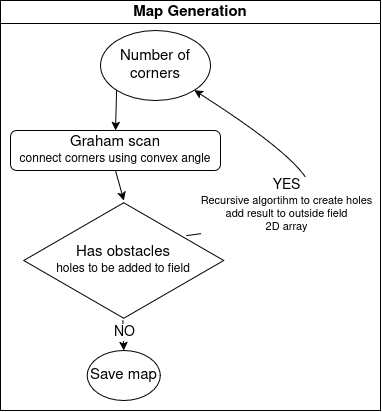
\includegraphics[width=0.5\textwidth]{./images/mapGen.drawio.png}
	\caption{Architecture of map generation}
	\label{MG:arch}
\end{figure}


Map generation is an important part of testing this system, it is important to test on all scenarios that may occur in the real world.
For this reason, random or parameter based map generation is very necessary to guarantee success in every environment.
As the outputs of this section will mostly be used for testing the path planning algorithm on regions with differing area, number of corners and complexity, no excessive algorithmic complexity is needed.
This program should also be able to create n obstacles within the main field, such areas would represent obstructions in the mowers desired path, for example trees or telephone poles in the real world.
This means we need a function with 2 parameters:

\begin{itemize}
	\item \textbf{K}, number of angles in the outer field
	\item \textbf{N}, number of obstacles within the field, since it would not be sensible to take a parameter for the number of corners for every hole, we can generate them randomly assuming 3–8 corners staying inline with the complexity of the rest of the field without being unreasonably overengineered.
\end{itemize}


\subsubsection{Corners}
The number and distance between corners could be thought to represent complexity of a shape.
It is important that both the number and placement of corners in a field are variable to simulate all situations that may occur in the real world.
This leads to robust and intense testing ensuring reliability in practice.


\subsubsection{Obstacles}
Obstacles or holes, can be thought to represent real world obstructions for example trees or telephone poles in a real field.
Generation of obstacles can be completed using the same function as the outer field generation, simply with different parameters.
The algorithm \ref{mg:genPoints} takes 3 parameters, number of points in the shape, an origin point and the range new points.
This allows for variable size, positioning and complexity.


\subsubsection{Graham Scan}
The Graham Scan \citep{graham1972efficient} is an algorithm to find convex hulls, that is from a set of points the outline which contains all inner points.
This algorithm does this by sorting the points by their polar angle to the lowest point, since this is always in the hull.
There is then further calculations based on the angle between adjacent points to omit inner points from the outline, however for this use case that is not necessary since all points will be vertexes in a field.
For this reason, the algorithm used is not strictly a Graham Scan but rather heavily based on the first stage, as shown in \ref{mg:sortPoints}
Using this algorithm allows for consistent outlining of any set of points with no crossovers or intersections

\subsection{Complete Coverage Path Planning}

\begin{figure}[H]
	\centering
	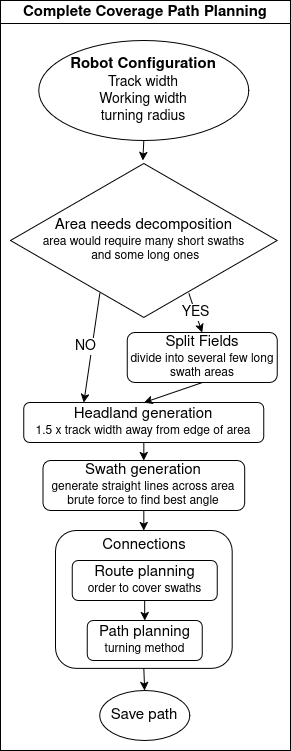
\includegraphics[width=0.4\textwidth]{./images/pathPlanning.drawio.png}
	\caption{Architecture of path planning process}
	\label{PP:arch}
\end{figure}


For this module, I have used the Fields2Cover library \citep{fields2cover}, this library is open source.
During the course of this project, I contributed to his library, fixing a bug during the build process.
The library splits the task up into several sub-tasks.


\subsubsection{Robot Configuration}
Robot sizing has 2 important factors, track width, how wide the machine itself is, and blade width, how wide the utility object is.
For farming equipment the utility object is usually larger than the vehicle, for example a combine harvester's wheels being narrower than blade, however for this project the blade is within the tracks.
For this reason the functions will compute slightly differently to its probable intended use case as the tracks are likely to overlap however this should not cause an issue and all outputs should function as needed.

The robot has 2 more parameters regarding its turning circle, these are minimum turning radius and maximum differential curvature.
Both of these are important when calculating a path for the robot to follow as they ensure the robot can easily follow the path.

The robot is 22cm wide from outer edge to edge and the gap between the tracks is 17cm, with a track width of roughly 2.5cm.


\subsubsection{Headland Generation}
Headlands are the area in which a vehicle turns, think of the rough edges of a crop field, these exist so that agricultural vehicles do not trample their crops when turning.
Although for the use case of a golf course this is not strictly needed as there are no "crops" or areas the robot cannot touch, so in this usecase headlands are not necessary.
Headlands can also generated around obstacles to allow for suitable turning area around the obstacles if needed, this serves as an area to do a "U-turn", effectively the same as reaching the end of the field.


\subsubsection{Swath Generation}
Swaths are the individual straight lines that make up the complete path,
they are often parallel to each other, but this can vary depending on how the shape of the field is segmented into smaller shapes however they will always be parallel while in the same sub area.
There are 2 ways of determining the optimal angle; the sum of the lengths of all swaths, or the number of swaths, where lower is better for each.
Both of these have pros and cons, for example lower total length offers better time efficiency assuming a near constant travel speed while lower swath count gives reduced turning movements which can be better if turning requires a slower speed or other complexities.
Similarly, lower sum length of course means less distance travelled and usually less fuel/energy consumed, however the opposite can be true if the acceleration and deceleration causes greater energy consumption compared to constant velocity.
Swaths are generated within the bounds of the headlands to allow for independent handling of the turning and connection of swaths regardless of the rest of the generation process.
To find the best angle, each angle is tested and compared. This brute force approach could be considered slow, but it is all the library offers and could be taken into consideration in a future release.

\subsubsection{Route Planning}
A route is the order in which swaths will be covered.
These can be sorted in a number of ways:

\begin{itemize}
	\item{\textbf{Shortest route} to cover all swaths, order depends on field}
	\item{\textbf{Boustrophedon order}, a zigzag like pattern covering swaths in order (1,2,3...)}
	\item{\textbf{Snake order}, Similar to Boustrophedon but skipping 1 swath each time (1,3,5...)}
	\item{\textbf{Spiral order}, a spiral pattern around the field, first swath then last (1, n, 2, n-1...)}
	\item{\textbf{Custom order}, user defined}
\end{itemize}
While they all ensure complete coverage, each of these has their benefits:

The shortest route method uses OR-Tools \citep{ortools} to compute the shortest route to cover all swaths, it considers headland paths and is the only method to do so.
While it will always find the quickest path, it also has the longest computation time due to the extra, sometimes complex mathematics involved.

Boustrophedon is the most efficient for rectangular shapes, traversing swaths in order minimising the number of turns and therefore wasted time and energy.

Snake order is the same as boustrophedon but provides a better solution when turning radius is large or multiple passes are needed to completely cover the area.


Spiral order can be benificial in irregular or circular areas where back and forth patterns cause a large number of unnecessary turns.
It also prevents going back over already covered areas which provides greater time efficiency.

Since all of these have their specific use cases it would not make sense to pick one for all appliactions, instead it should be considered for each generation by the user.

\subsubsection{Path Planning}
Path planning refers to the connection of all swaths in route order.
There are a couple of ways the to link neighbouring swaths: the \textbf{Dubins curve} and the \textbf{Reeds-Shepp curve}.

% \begin{itemize}
% 	\item{Dubins Curve}
% 	\item{Reeds-Shepp curve}
% \end{itemize}

Both of these compute the shortest path between the 2 points, with the deciding factor between the 2 being the robots' ability to move backwards.
Reeds-Shepp allows backwards movement which can be helpful when headlands are not needed, allowing for mowing right to the edges of an area.

There is a derivative of both of these featuring continuous curvature, this substitutes a slightly longer path for a wider turning angle but higher average speed.
The advantages of continuous curvature are mainly for vehicles that have difficulty turning sharply.

However, since the robot moves on tracks, it can turn in place.
This means the majority of benefits for path planning techniques are invalid, instead the most time is saved by having the shortest path and least angle to turn on the spot.
So the best method for this use case is likely the Reeds-Shepp as it can work with no headland and produces nearly straight lines for its links between swaths.


\subsubsection{Cell Decomposition}
For shapes with unusual shapes, a large "L" shape for example see \Cref{ccpp:cellDecomp}, constant swath angle can be problematic.
The simple fix for this issue is to treat both sections of fields as separate objects planning coverage optimally for each "straight".
This method of abstraction is responsible for huge saving in both processing mowing time due to reducing the amount of unnecessary swaths and turns.

\subsubsection{Final Setup}

\begin{itemize}
	\item{\textbf{Mower size}, 0.22m track wide, 0.15m working width}
	\item{\textbf{Headland generation}, no headlands - full coverage}
	\item{\textbf{Swath generation}, brute force - optimal pathing}
	\item{\textbf{Path planning}, Reeds-Shepp curve - minimizes time off of course}
	\item{\textbf{Route planning}, shortest route - seems to minimize time out of area too}
\end{itemize}



\subsection{Aerial Map Generation}
Previously, for the program to take in a real world map from an image of the real world, the user would have to upload the picture and manually trace the outline, this could cause some problems.
For example, the outline is only as accurate as the user's mouse placement, likely skipping some smaller corners to save time or due to inability to be accurate to the necessary degree.
Automating this laborious and time-consuming task would positively increase user experience and usability, this can be done using algorithmic and machine learning approaches.

\subsubsection{Algorithmic Approaches}


\begin{figure}[H]
	\centering
	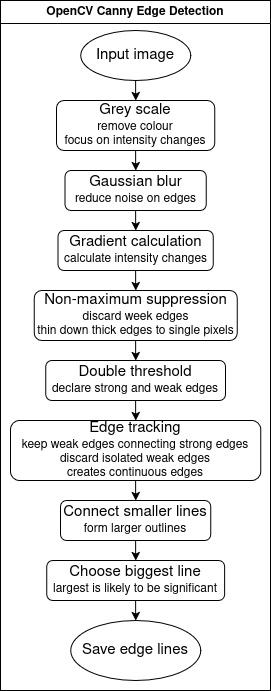
\includegraphics[width=0.35\textwidth]{./images/openCV.drawio.png}
	\caption{Architecture of map generation}
	\label{AE:openCVarch}
\end{figure}



There are several algorithmic methods that try to achieve this task from several different librarys. A popular library for image processing is OpenCV\citep{opencv_library}.

OpenCV's Canny edge detection implementation follows the classic algorithm developed by Canny \citep{canny1986computational}.
The algorithm works through several steps to detect edges in images:
\begin{itemize}
	\item \textbf{Grayscale Conversion}: 
	\item \textbf{Gaussian Blur}: First, the image is smoothed with a Gaussian filter to reduce noise, as edge detection is highly sensitive to noise.
	\item \textbf{Gradient Calculation}: The algorithm calculates the intensity gradients of the image using Sobel filters in both horizontal and vertical directions:
	\item \textbf{Non-maximum Suppression}: This step thins out the edges by keeping only the local maxima. For each pixel, it checks if it's a local maximum in the direction of the gradient. If not, it's suppressed (set to zero).
	\item \textbf{Double Thresholding}: The algorithm applies two thresholds:
	      \begin{itemize}
		      \item High threshold: Pixels above this are considered "strong" edges
		      \item Low threshold: Pixels between low and high are considered "weak" edges
	      \end{itemize}
	\item Edge Tracking by Hysteresis: Finally, weak edges that are connected to strong edges are kept, while isolated weak edges are discarded. This helps ensure that the detected edges are continuous.
\end{itemize}
This approach works very well for high contrast images, particularly those black and white~\Cref{am:cannyexample}. The clear separation between foreground and background elements allows the algorithm to detect distinct gradient changes and create clean, continuous edge lines.

As for the similarly coloured golf course images, it can often find the outlines but they are made up of many smaller lines~\Cref{am:CannyGolfCourse}. This fragmentation occurs because the subtle color transitions between different areas of the golf course (like fairways, roughs, and greens) create weaker gradient signals that may fall inconsistently above or below the detection thresholds.

It may appear there is a simple solution to this problem; join the connected lines into one, however this proves to be rather problematic in itself for a number of reasons:

\begin{enumerate}
	\item The desired line does not form a complete shape - Gaps in the detected edges mean that even sophisticated line-joining algorithms may fail to connect all segments belonging to a single boundary

	\item The line is connected to other lines outside the desired shape - Many detected edges from shadows, texture variations, or other regions of the golf course can intersect with the boundary edges required to be isolated, creating unwanted connection points

	\item Once lines are connected, it is impossible to tell which collection of lines is needed - Without prior knowledge of the expected shape or additional contextual information, there's no reliable way to determine which edge segments represent meaningful boundaries, like the edge of a green compared to an outline of trees or a rough area.
\end{enumerate}
All of these means use of canny edge detection can often cause more problems than it solves, while it may have more accurate outlines in places, they may be connected to unwanted areas, Or they may not be complete and still require further user input to chose a selection or finish a shape.

\subsubsection{Machine Learning Approach}

\begin{figure}[H]
	\centering
	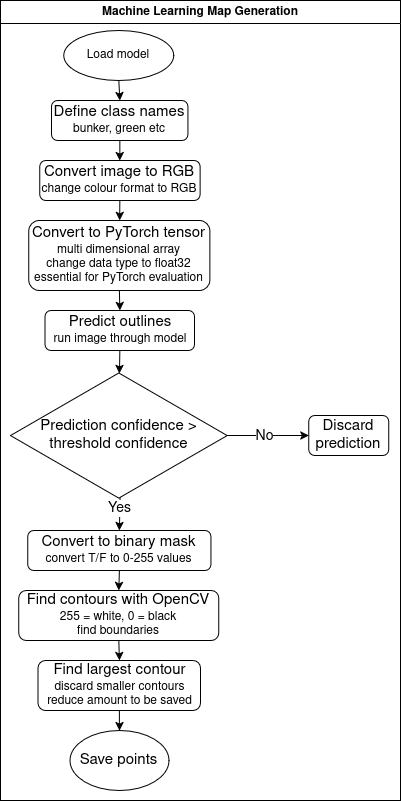
\includegraphics[width=0.35\textwidth]{./images/MLAE.drawio.png}
	\caption{Architecture of map generation}
	\label{AE:MLAE}
\end{figure}

Another possible solution to this problem is to use a machine learning network to predict the areas of the golf course.
PyTorch \citep{pytorch} is a powerful open-source machine learning library and has become one of the most popular frameworks for deep learning research and production applications since its initial release in 2016.
It was developed to show that usability and speed can both be present in a python implementation of machine learning making it the perfect tool for this task.

\paragraph{Model} \

For this specific problem, a Mask R-CNN model is best.
Mask R-CNN models offer strong instance segmentation meaning they are good for outline individual parts of images to within pixels of accuracy and therefore greater precision.
This type of model is ideal for golf courses since they can distinguish between the similarly coloured parts of a golf course e.g. bunkers vs fairway.

\paragraph{Data Set} \

A models training data needs to be closely related to its real world input data, for the Robot Mower that is satellite and drone images or orthophotos from above the desired mowing area.
Training data also needs to be clearly and consistently annotated to produce accurate, reliable results in practice.
The only orthophoto data set publicly available is the danish golf course data set \citep{danishgolf}, a dataset produced by the Danish government, however common annotations lack quality and consistency; the outlines do not cover the whole area of single sections and often are missing entirely.
Upon testing the data with these annotations, it produced faulty results including both true negative and false positives ~\Crefrange{am:AGDanish}{am:ohGCDanish}.
However, since the raw orthophotos are still highquality images, they are still suitable inputs but will require custom annotations.

Labelme \citep{labelme} is an open source python adaptation of an older tool produced originally by MIT allowing users to draw around parts of an image creating boundaries and saving them as a list of points in a \textbf{.JSON} format.

To avoid over training on specific regions a mix of golf course images were going to be used in the training data including some images form the Danish date set, Google Earth and various other sources.
This was in an attempt to promote more diverse predictions from data with different shadow angles, grass colour and design.
However, in practice the vast range of shades and colours was a weakness rather than a strength.
Results with this larger dataset lead to unreliable results across all tests on data that was and was not used in the training phase, see ~\Cref{am:AEEnglishCourseResult}, the result of a golf course in England, featuring much darker greens than the large proportion Danish training data.
To fix this it seemed that region specific specialisation was needed which for the reasons mentioned above made sense to be Denmark based golf courses.

One prominent issue with this data set, and probably any data golf course image for that matter, is that bunkers are far more common than any other class.
This can cause overprediction of bunkers while causing unbalanced results and greater uncertainty for other classes.
The remedies to this issue are simply more training data and to implement a class weighting system in training and prediction.

Doubling the data count caused slightly more consistency while adding class weights was a game changer.
Class weights adjusted for the less frequent classes like fairways and greens but still not enough for rough as seen in ~\Cref{am:AENoRoughDemoTraining}.
The lack of rough in this instance was because in most cases, they are large single annotations unlike the frequent smaller bunkers which are predicted with very low uncertainty.
Breaking up roughs into smaller sections covering the same area increases the frequency and diversifies the characteristics, progressing towards a more balanced situation for the same reason bunkers are predicted with high accuracy.

\paragraph{Training} \

% Tracks stats for each class(pixel area, count) > sample weights - boosts rare classes
The training process is important when considering a good model. 
Appropriate parameters are needed to ensure good learning and correction, the following are some parameters used in this training loop.
Each class' statistics are tracked such as number of occurrences and total pixel area, these values are used to adjust the weighting during training to improve accuracy and reduce uncertainty of each class.
To account for the less common classes such as water features, images containing these are trained on more often with their weights boosted to ensure each class is well represented in the learning.
Similar weighting is used in the loss function of each class to further emphasise their rarity, this is inaccurate prediction of less frequent classes hold a greater penalty than more frequent ones.
Boosting exposure to rarer classes like this means the model is well-equipped to identify them if they do occur in real world use.
The accuracy and loss of each class is also taken into consideration to further adjust things if needed.

Random transformations are used to increase the robustness of the model, these can happen in a number of ways:

\begin{itemize}
	\item{Horizontal flipping}
	\item{Colour jitter}
	\item{Rotiation}
\end{itemize}
Using the same images with slight adjustments increases reliability and should allow the model to work well on images with varying quality but also real world factors like shadowing or sun angle, without needing a great increase in the size of the dataset.

The model starts with PyTorch's \textbf{maskrcnn\_resnet50\_fpn} architecture with pretrained weights on the COCO \citep{coco} dataset.
This model serves as a strong backbone as it produces high accuracy in segmentation tasks while simultaneously being able to quickly learn on new domains.
Its RoIAlign layer features pixel to pixel mapping between input images and masks predictions resulting in much finer boundaries that previous generations.

As is typical for machine learning, the dataset is split into 2 parts for each training epoch. 80\% for training and 20\% for validation to get an approximate score of the current parameters.
This approach allows for constant iteration and adjustment on the fly resulting in faster training times and a better final model.

The model uses an early stop method to save more time when possible, as mentioned before the loss of each epoch is tracked if the loss does not improve over a set number of epochs, in this case \textbf{20}, training is ceased and the best model is saved.
This prevents unnecessary training cycles when aiming for a set number of epochs.


\paragraph{Basic Evaluation} \

With a complete data set and the outlines parameters above, these are some current performance metrics of the resulting model.

\begin{table}[H]
\centering
\begin{tabular}{c|c}
\hline
\textbf{Overall Metric} & \textbf{Value} \\
\hline
\hline
Overall Precision & 0.7035 \\
Overall Recall & 0.7943 \\
Overall F1-Score & 0.7462 \\
Mean IoU & 0.7934 \\
Pixel Accuracy & 0.7718 \\
Total Detections & 1383 \\
Total Ground Truth & 1225 \\
\hline
\end{tabular}
\caption{Overall Model Performance Metrics}
\label{tab:overall_metrics}
\end{table}


\begin{table}[H]
\centering
\begin{tabular}{c|c|c|c|c|c|c|c}
\hline
\textbf{Class} & \textbf{Precision} & \textbf{Recall} & \textbf{F1-Score} & \textbf{IoU} & \textbf{TP} & \textbf{FP} & \textbf{FN} \\
\hline
\hline
Green & 0.7449 & 0.8679 & 0.8017 & 0.8760 & 184 & 63 & 28 \\
Fairway & 0.8092 & 0.8327 & 0.8208 & 0.7933 & 229 & 54 & 46 \\
Bunker & 0.9197 & 0.8253 & 0.8700 & 0.8371 & 378 & 33 & 80 \\
Rough & 0.3811 & 0.6230 & 0.4729 & 0.5743 & 157 & 255 & 95 \\
Water & 0.8333 & 0.8929 & 0.8621 & 0.9025 & 25 & 5 & 3 \\
\hline
\end{tabular}
\caption{Per-Class Detailed Performance Metrics}
\label{tab:class_metrics}
\end{table}


Where each term is defined as follows:
\begin{itemize}
    \item \textbf{Precision}: The proportion of correctly predicted positive instances out of all instances predicted as positive.\\
    Formula: $\displaystyle \text{Precision} = \frac{TP}{TP + FP}$

    \item \textbf{Recall} (Sensitivity or True Positive Rate): The proportion of correctly predicted positive instances out of all actual positive instances.\\
    Formula: $\displaystyle \text{Recall} = \frac{TP}{TP + FN}$

    \item \textbf{F1-Score}: The harmonic mean of Precision and Recall, used to balance both metrics.\\
    Formula: $\displaystyle \text{F1} = 2 \times \frac{\text{Precision} \times \text{Recall}}{\text{Precision} + \text{Recall}}$

    \item \textbf{IoU (Intersection over Union)}: Measures the overlap between the predicted and actual bounding boxes in object detection.\\
    Formula: $\displaystyle \text{IoU} = \frac{\text{Area of Overlap}}{\text{Area of Union}}$

    \item \textbf{TP (True Positive)}: The model correctly predicts the positive class.

    \item \textbf{FP (False Positive)}: The model incorrectly predicts the positive class.

    \item \textbf{FN (False Negative)}: The model fails to predict the positive class when it should have.
\end{itemize}


\subsection{Post Processing}

\begin{figure}[H]
	\centering
	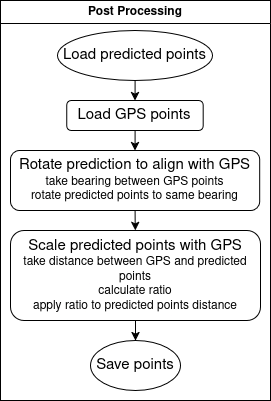
\includegraphics[width=0.35\textwidth]{./images/postProcessing.drawio.png}
	\caption{Architecture of map generation}
	\label{PPr:arch}
\end{figure}

After the aerial map has been generated, there are a few more steps to take to ensure geographical accuracy.
The map must align with the field for the path to be accurate.

To do this some real world GPS or RTK coordinates are needed.
The minimum number of required points is 2, representing the first 2 corners of the intended area, from just 2 points the rotation and scale can be determined.

The map is corrected to real world bearing and size by matching coordinates to their corresponding vertices of the map.
The bearing and distance between GPS points is translated to every point of the predicted map producing an accurate representation of the real area which is then saved.


\subsection{User Interface}
To bring all components listed in this report together, a simple graphical user interface is needed.

This GUI features buttons to load images for the machine learning model and begin the process, a checkbox to scale with real coordinates and a progress bar displaying the progress of the system.


\begin{figure}[h!]
	\centering
	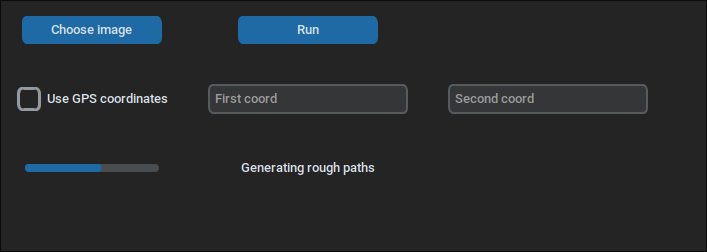
\includegraphics[width=0.5\textwidth]{./images/GUI.png}
	\caption{Screenshot of GUI for this program}
	\label{GUI}
\end{figure}

\section{Performance Evaluation}

Performance is a key part of user experience therefore is crucial to the real world performance of this product.
Performance in this case can be broken down into 2 key metrics:

\begin{itemize}
	\item{\textbf{Run time}: how long the process takes to complete in real time}
	\item{\textbf{Memory Usage}: how much system memory the process uses both average and maximum}
\end{itemize}

Both of these can be measured in python consistently and reliably, meaning the code can be directly tested in the same file without needing system usage or other programs that may have their own overheads.
Each module will be run with different parameters to see how they impact performance which then will be run 5 times,
these 5 results will then be averaged and plotted against the chosen parameter providing clear graphs to visualise any impact varying inputs may have on the products performance.
A baseline run will be provided using set parameters and run 10 times to show a good default.

Run time will be measured in milleseconds and track the total execution time from start to finish.
The tool used to measure exectuion time  is the \textbf{time} library and its \textbf{perf\_counter} function.
This is accurate to nanoseconds and causes negligable difference in runtime.

Memory Usage will be measured in MB and track the average and peak memory usage during the runtime of the program.
Peak memory usage is tracked using the \textbf{tracemalloc} library.
This library tracks the peak memory usage of the code exectuion.

For reference, these benchmarks were taken on a \textbf{Ryzen5 5600X} with \textbf{16GB} of R.A.M. at \textbf{3200 MT/s} and where relevent \textbf{GeForce RTX 3060 Ti}.

\subsection{Map Generation}
\subsubsection{Run Time}
\paragraph{BaseLine} \

\Cref{PE:mg:baselineRT} represents the baseline and tested with 10 corner points, 0-400 range and 0 holes.
The runtime is fairly consistent having a very small range of 0.2 milleseconds, showing a very strong baseline to run further testing on.


\paragraph{Number of points} \

\Cref{PE:mg:points} shows the impact of varying the number of points on runtime.
The tests were run with a range or 0-400 and 0 holes.
Clearly points are added in linear respect to execution time but are efficient in doing so, taking around 0.0075 milleseconds per point added.
Points are added with O(n) complexity


\paragraph{Range of points} \

\Cref{PE:mg:range} visualises the time taken when varying limits are placed on the range of points, this can be thought to represent the Physical size of the field.
These runs were carried out with 10 points and 0 holes.
There is no clear correlation between the range of points and the run time of the program, the graph closely resembles the baseline, having the same range and very similar bounds at each side.
The quickest runtime from this test and all baseline runs actually occurs with a range 1200, three times the range in the baseline.
This is a very good indication on top of everything else that range has no effect on runtime meaing the program should work for any size of field in good time.

\paragraph{Number of holes} \

\Cref{PE:mg:holes} demonstrates how the number of holes translate to runtime.
The runs were carried out with 10 points in the main field, a range of 400 and 5 points in each hole.
Similarly to the number of points, the number of holes has a linear effect on runtime, however runtime increaes in larger steps.
This is likely because in this example, each hole has 5 points and an extra append operation, this is likely why the same number of points generated in the outside field, and in total considering holes differ in runtime.
For instance, 200 points in a single field takes around 1.5ms but 210 points comprised of 10 in the outer field and 40, 5 point holes just under 2ms.
This time increase does not line up and could be for a number of reasons such as the additional appending to the array or the random number generation process of the point generation function, or could be the extra overheads from the sorting of the points in each hole.
Whichever of these is the cause, or if it is a combination of all 3, they are all needed operations so nothing can be done to improve this further, although they whole process still completes in an insignificant amount of time, even with 200 holes it only takes around 9 milleseconds.
200 holes is likely far more than any real world appliaction would need but still computes in excellent time.


\subsubsection{Memory Usage}

\paragraph{Baseline} \

\Cref{PE:mg:memBaseline} is a baseline graph to show the memory usage of the map generation process with 10 points, 400 range and 0 holes.
There memory usage is quite consisten except for the obvious outlier on run 1.
There is no clear reason for this but it occured on every measurement taken, it is possible it is an issue with the measurement script although unlikely.


\paragraph{Number of points} \

\Cref{PE:mg:memPoints} shows the memory usage of the map generation process with variable points, 400 range and 0 holes.
Points effect memory linearly which make sense as there is contasnt size need for each point.
The amount of memory needed is very small and is almost guaranteed to be suitable for any computer system even a low end portable micro PC such as a raspberry Pi.


\paragraph{Range of points} \

\Cref{PE:mg:memRange} draws the memory usage of the map generation process with 10 points, variable range and 0 holes.
Increasing the range of points does have a positively correlated effect on memory when compared to the baseline.
This could be for a number of reasons but essentially comes down to the higher number possible coordinate values.
That could be the data structure of the point takes more memory to store the greater value, because the random number generation process requires more memory or becuase the sorting algorithm needs to memory to sort the higher values.

\paragraph{Number of holes} \

\Cref{PE:mg:memHoles} demonstrates the memory usage of the map generation process with 10 points, 400 range and variable holes.
As mentioned in the runtime section, holes are closely related to points, they effect memory linearly, but at a higher rate than points as they are a collection of points.
Where memory differs to runtime however, is there are no overheads to having points as holes or a single field, since memory allocation is constant.
This concludes the number of holes is irrelevant and the number of total points is all that needs to be considered.


\subsection{Complete Coverage Path Planning}
\subsubsection{Runtime}
\paragraph{Baseline} \

\Cref{PE:p:BaselineRT} shows a baseline runtime for the fields2cover library generating with:

\begin{itemize}
	\item{\textbf{Area}, $10^3\,\text{m}^2$ and 6 sides}
	\item{\textbf{Mower size}, 0.22m track wide, 0.15m working width}
	\item{\textbf{Headland generation}, constant function}
	\item{\textbf{Swath generation}, brute force}
	\item{\textbf{Route planning}, boustrophedon order}
	\item{\textbf{Path planning}, dubins curve}
	\item{\textbf{Cell decomposition}, none}
\end{itemize}
These paremters are all default, first mentioned or most simplistic to give a stable baseline.

\paragraph{Map Size} \

\Cref{PE:p:SizeRT} shows how differing field size affects the runtime of algorithm.
The graph shows an exponential relationship between the two, this makes sense because there are a number of components affected by field area:

\begin{itemize}
	\item{Area calculations}
	\item{Buffer operations, used to generate headland}
	\item{Swath generation and optimal angle}
\end{itemize}
All of these cause longer runtimes on larger areas, mostly due to the increase of calculation complexity or simply needing more calculations to complete the process.
The graph shows upto 10^5m^2$ which is about the size of 14 football pitches, taking about 8 seconds.
While this is a long time to wait, it is unlikely that the program will have to consider an area this large very often since most input images are going to be close up to capture detail.


\paragraph{Route Planning Method} \

\Cref{PE:p:RoutePlanningRT} shows how different route planning methods impact processing time.
There is not much difference betwen the 3 known patterns, almost margin of error, but the shortest route method takes much longer.
This is because, the 3 knowns requrie 0 calculations just simple array indexing in a set order.
Where as the shortest route method uses a brute force approach and requires vast calculations to find the best sequence, this time increase is also likely to have a non linear affect when paired with larger fields.

\paragraph{Number of Holes} \

\Cref{PE:p:HolesRT} Shows how the number of holes in a field affect the overal run time, this test was conducted on an 80 x 80 square field with a varying number of holes.
When holes are present, the \textbf{Shortest Route} planning method must be used to connect the isolated swaths that border obstacles and as seen above this going to impact run time on its own, so it is expected that runtime will be longer than before.
Holes have a linear effect on run time, this makes sense as field generation and swath placement is linear.


\subsubsection{Memory Usage}

\paragraph{Baseline} \

The baseline graph \Cref{PE:p:BaselineMem} indicates constant memory usage across several executions of the pathing method.
This consistency in results indicates a stable process for path generation that should be reliable and produce identical results each time it is required.

\paragraph{Map Size} \

According to \Cref{PE:p:SizeMem}, field area has very little impact on the memory consumption.
There seems to be 3 levels of memory consumption but it is unclear which parameter causes the discrepancy since the results are not in distinct groups.
The range is within 30 bytes of each other, this small variation is completely normal and is likely unavoidable due to the nature of python's memory allocation system.
The results of this test are negligable and can be considered consistent within a working margin.



\paragraph{Route Planning Method} \

\Cref{PE:p:RoutePlanningMem} displays the peak memory usage when using different route plannig methods. Yet again, memory usage is hardly changed by the selected method, this seems strange especially for the shortest route application since there are so many calculations and processing overheads.
The short range is a big positive and allows the route planning decision can be made purely on runtime and physical factors without worrying about system limitations, aslong as processing runtime is not a huge concern, shortest route can be used bringing big benefits to the physical use.



\paragraph{Number of holes} \

\Cref{PE:p:HolesMem} shows the peak memory vartation with differing number of holes in the field.
As mentioned in the runtime test the map for this test is slightly different, taking place on a 80x80 sqaure field with a number of sqaure holes, this approach is necessary to ensure consistent placement of holes in the field.
The results show 2 things; the number of obstacles in a field do not affect memory and memory consumption is not directly affected by the shape of the field.
Both of these are good results and show memory is largely similar accross any selection of parameters, consistently low memory usage is a very good trait for an embedded system such as this, meaining computation can be carried out on a variety of computers with differing specfications, specifically low spec end micro computers.

\subsection{Aerail Map Generation}
The metrics taken from the machine learning aerial mapping model were:
\begin{itemize}
    \item{\textbf{Pixel Accuracy:} the percentage of pixels assigned the correct class by the model}
    \item{\textbf{Quality Detection Accuracy:} the percentage of objects in an image correctly predicted with good segmentation, e.g. number of bunkers or greens}
\end{itemize}
Both of these were tested against serveral parameters as follows.

\subsubsection{Confidence Threshold} \label{confidenceThresholdEval}

Confidence threshold is the needed degree of certainty for the outputs of the model to be considered.

Results of this section are shown in (\Cref{AE:Confidence})

\paragraph{Pixel Accuracy} \

The graph shows a non linear relationship between the pixel accuracy and confidence threshold, peaking at around 0.6 confidence, this signifies the model is over estimating areas at the low end \textbf{0 - 0.4}, fairly accurate in the mid range \textbf{0.5-0.8} and too strict at the upper end \textbf{0.9 - 1}.
The accuracy peaks at around \textbf{0.6} so this is the confidence level that will be used going forward.

\paragraph{Detection Accuracy} \
The relationship between detection accuracy and confidence threshold is an almost linear negative correlation.
The probable cause of this is as confidnce threshold increaes, less predicitions are passing the threshold.
The sharp drop suggests the model is not very confident with the majority of its predictions, this is likely to be helped with additional training data.



\subsection{Intersecion over Union (IoU)}
Intersection over union is the overlap between the ground truth and area predicted by the model.
There are 2 types of IoU measurement that can be used during evaluation of an image processing model:

Bounding box IoU a box around the outer points of the ground truth and prediction.
This concept helps to get direct overlapping area.

Mask IoU that only counts the predicted area. This offers more precise calcutions and is the chosen option for the following tests.

Note that the x axis on these graphs stop at \textbf{0.9}, this is because a IoU of \textbf{1} is nearly impossible for a task as complex as this so would nearly always equal \textbf{0}. For this reason it has been omitted to allow a higher detail reading of the graphs.

Results for this paremter can be seen in (\Cref{AE:IOU})

\paragraph{Pixel Accuracy} \

As with the confidence threshold a non linear relationship can be seen with a peak around the mid range, in this case \textbf{0.6}, again likely due to this being the sweet spot where the model is close enough to the ground truth without being too restricted in its outputs.

\paragraph{Decection Accuracy} \

The relationship between the threshold  IOU to detection accuracy seen in the graph shows that lower IoU causes higher detection rates.
This is most likely because lower IoU allows the model to be less precise in location with predictions, however this it is probable that this would cause lower pixel accuracy due to the more relaxed location. 


\section{Conclusion and Future Work}


Another essential section that should keep its title as suggested. Briefly discuss your main findings, outcomes, results; what worked and what could have been done differently. Then summarise your work in a concluding statement by comparing your outcomes against the main and sub-objectives and/or MoSCoW requirements (if used) and suggest potential future work that could be done if more time would be available.

\subsection{Conclusion}
This report outlines the development of a new route planning system for an automated golf course mowing robot. 

The first step in this process is creating a map of an area from an aerial image using a maskRCNN machine leaning model trained.
This phase currently specialises in Dansih golf courses due the abundance of high quality orthophotos for this region, since shades, colour and other patterns can vary a specialisation on one region was necessary.
The output of the model is transformed to a real world orientation of the area based on several manual GPS coordinates.

The next step is complete coverage path planning on the transformed area.
This uses a brute force method to find optimal travel angles and hole detection is utilised to avoid areas that are untraversable for the robot such as sand bunkers or areas where the robot would need to use a different cutting setting for example on rough areas vs green that require a finer cut.

The user interacts with this through a clean and minimal graphical user interface.


\subsection{Future Work}

The current state of the project is a good baseline for future development but still has room for several improvements.

One such improvement could be collecting high quality training data representing other regions. UK golf courses typically consist of deeper greens with more distinct shades between the areas of a golf course. A seperate dataset could be developed, then allowing the user to manually select a region or automatically detect the better result.

Another adaptation could be agricultural use. 
Since Fields2Cover, the path planning library used in this project, is made with agriculture in mind if the mapping model was adapted the system could yield good results for a seperate use case to the current implementation.

A more complex GUI would be a good addition in increase the user experience with the product. The current one was rather an after thought than a core piece of the software but it is important that the user can interact with the program easily and intuitively.



\clearpage

\bibliography{reportbib}

\appendix
\clearpage

\section{Map Generation}

\begin{algorithm}[h!]
	\caption{Point Class Definition}
	\label{mg:point class}
	\begin{algorithmic}[1]
		\Procedure{class Point}{}
		\State $X \gets -1$ \Comment{X-coordinate initialized to -1}
		\State $Y \gets -1$ \Comment{Y-coordinate initialized to -1}
		\State $angle \gets -10$ \Comment{Angle initialized to -10}
		\Procedure{Constructor}{$x$, $y$}
		\State $this.X \gets x$
		\State $this.Y \gets y$
		\State $this.angle \gets -10$ \Comment{Default angle value}
		\EndProcedure
		\EndProcedure
	\end{algorithmic}
\end{algorithm}

\begin{algorithm}[h!]
	\caption{Generate random points}
	\label{mg:genPoints}
	\begin{algorithmic}[1]
		\Function{GenPoints}{$num$, $P$, $size$}
		\State $points \gets []$
		\For{$i \gets 0$ \textbf{to} $num - 1$}
		\State $randX \gets \text{random\_integer}(P.X + 1, P.X + size)$
		\State $randY \gets \text{random\_integer}(P.Y + 1, P.Y + size)$
		\State $points.\text{append}(\text{Point}(randX, randY))$
		\EndFor
		\State \Return $points$
		\EndFunction
	\end{algorithmic}
\end{algorithm}

\begin{algorithm}[h!]
	\caption{Sort points by polar angle to origin}
	\label{mg:sortPoints}
	\begin{algorithmic}[1]
		\Function{SortPoints}{$points$, $origin$}
		\State $hull \gets [origin]$
		\State Sort $points$ by Y-coordinate
		\For{$i \gets 0$ \textbf{to} $\text{length}(points) - 1$}
		\State $points[i].angle \gets$ \Call{CalcAngle}{$origin$, $points[i]$}
		\EndFor
		\State Sort $points$ by angle
		\State Append $points$ to $hull$
		\State \Return $hull$
		\EndFunction
	\end{algorithmic}
\end{algorithm}

\begin{algorithm}[h!]
	\caption{Main function}
	\label{mg:main}
	\begin{algorithmic}[1]
		\Function{Main}{}
		\State $hull \gets []$
		\State $origin \gets \text{Point}(20, 20)$
		\State $field \gets$ \Call{GenPoints}{$20$, $origin$, $400$}
		\State $hull.\text{append}($\Call{SortPoints}{$field$, $origin$}$)$
		\EndFunction
	\end{algorithmic}
\end{algorithm}

\begin{algorithm}[h!]
	\caption{Main function with holes in shape}
	\label{mg:mainWithHoles}
	\begin{algorithmic}[1]
		\Procedure{Main}{}
		\State $hull \gets$ empty list

		\State $origin \gets \text{Point}(20, 20)$
		\State $field \gets \text{GenPoints}(20, origin, 400)$
		\State add $\text{SortPoints}(field, origin)$ to $hull$

		\State $hole1Base \gets \text{Point}(100, 100)$
		\State $hole1Points \gets \text{GenPoints}(5, hole1Base, 50)$
		\State add $\text{SortPoints}(hole1Points, hole1Base)$ to $hull$

		\State $hole2Base \gets \text{Point}(150, 50)$
		\State $hole2Points \gets \text{GenPoints}(3, hole2Base, 30)$
		\State add $\text{SortPoints}(hole2Points, hole2Base)$ to $hull$
		\EndProcedure
	\end{algorithmic}
\end{algorithm}

\clearpage
\section{Complete Coverage Path Planning}

\begin{figure}[h!]
	\centering
	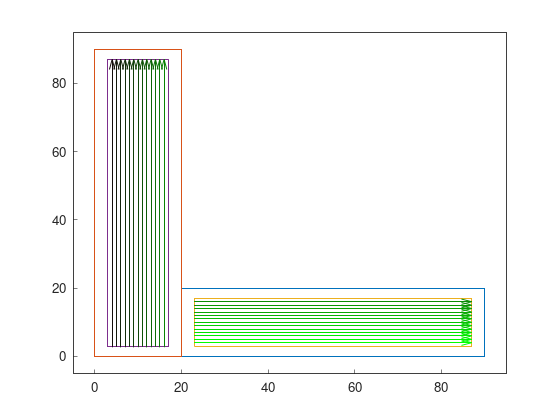
\includegraphics[width=0.6\textwidth]{./images/f2cCellDecompL.png}
	\caption{Example of an L shaped field where cell decomposition is optimal, taken from Fields2Cover docs}
	\label{ccpp:cellDecomp}
\end{figure}

% \clearpage
\section{Aerial Mapping}

\begin{figure}[h!]
	\centering
	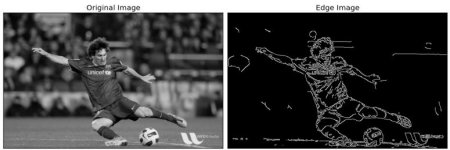
\includegraphics[width=0.7\textwidth]{./images/openCvCannyExample.jpg}
	\caption{Opencv example of canny detection, source \citep{opencv_library} docs}
	\label{am:cannyexample}
\end{figure}


\begin{figure}[h!]
	\centering
	\includegraphics[width=0.7\textwidth]{./images/openCvCannyGolfCourse.png}
	\caption{OpenCV canny edge detection on an image of a golf course}
	\label{am:CannyGolfCourse}
\end{figure}

\begin{figure}[h!]
	\centering
	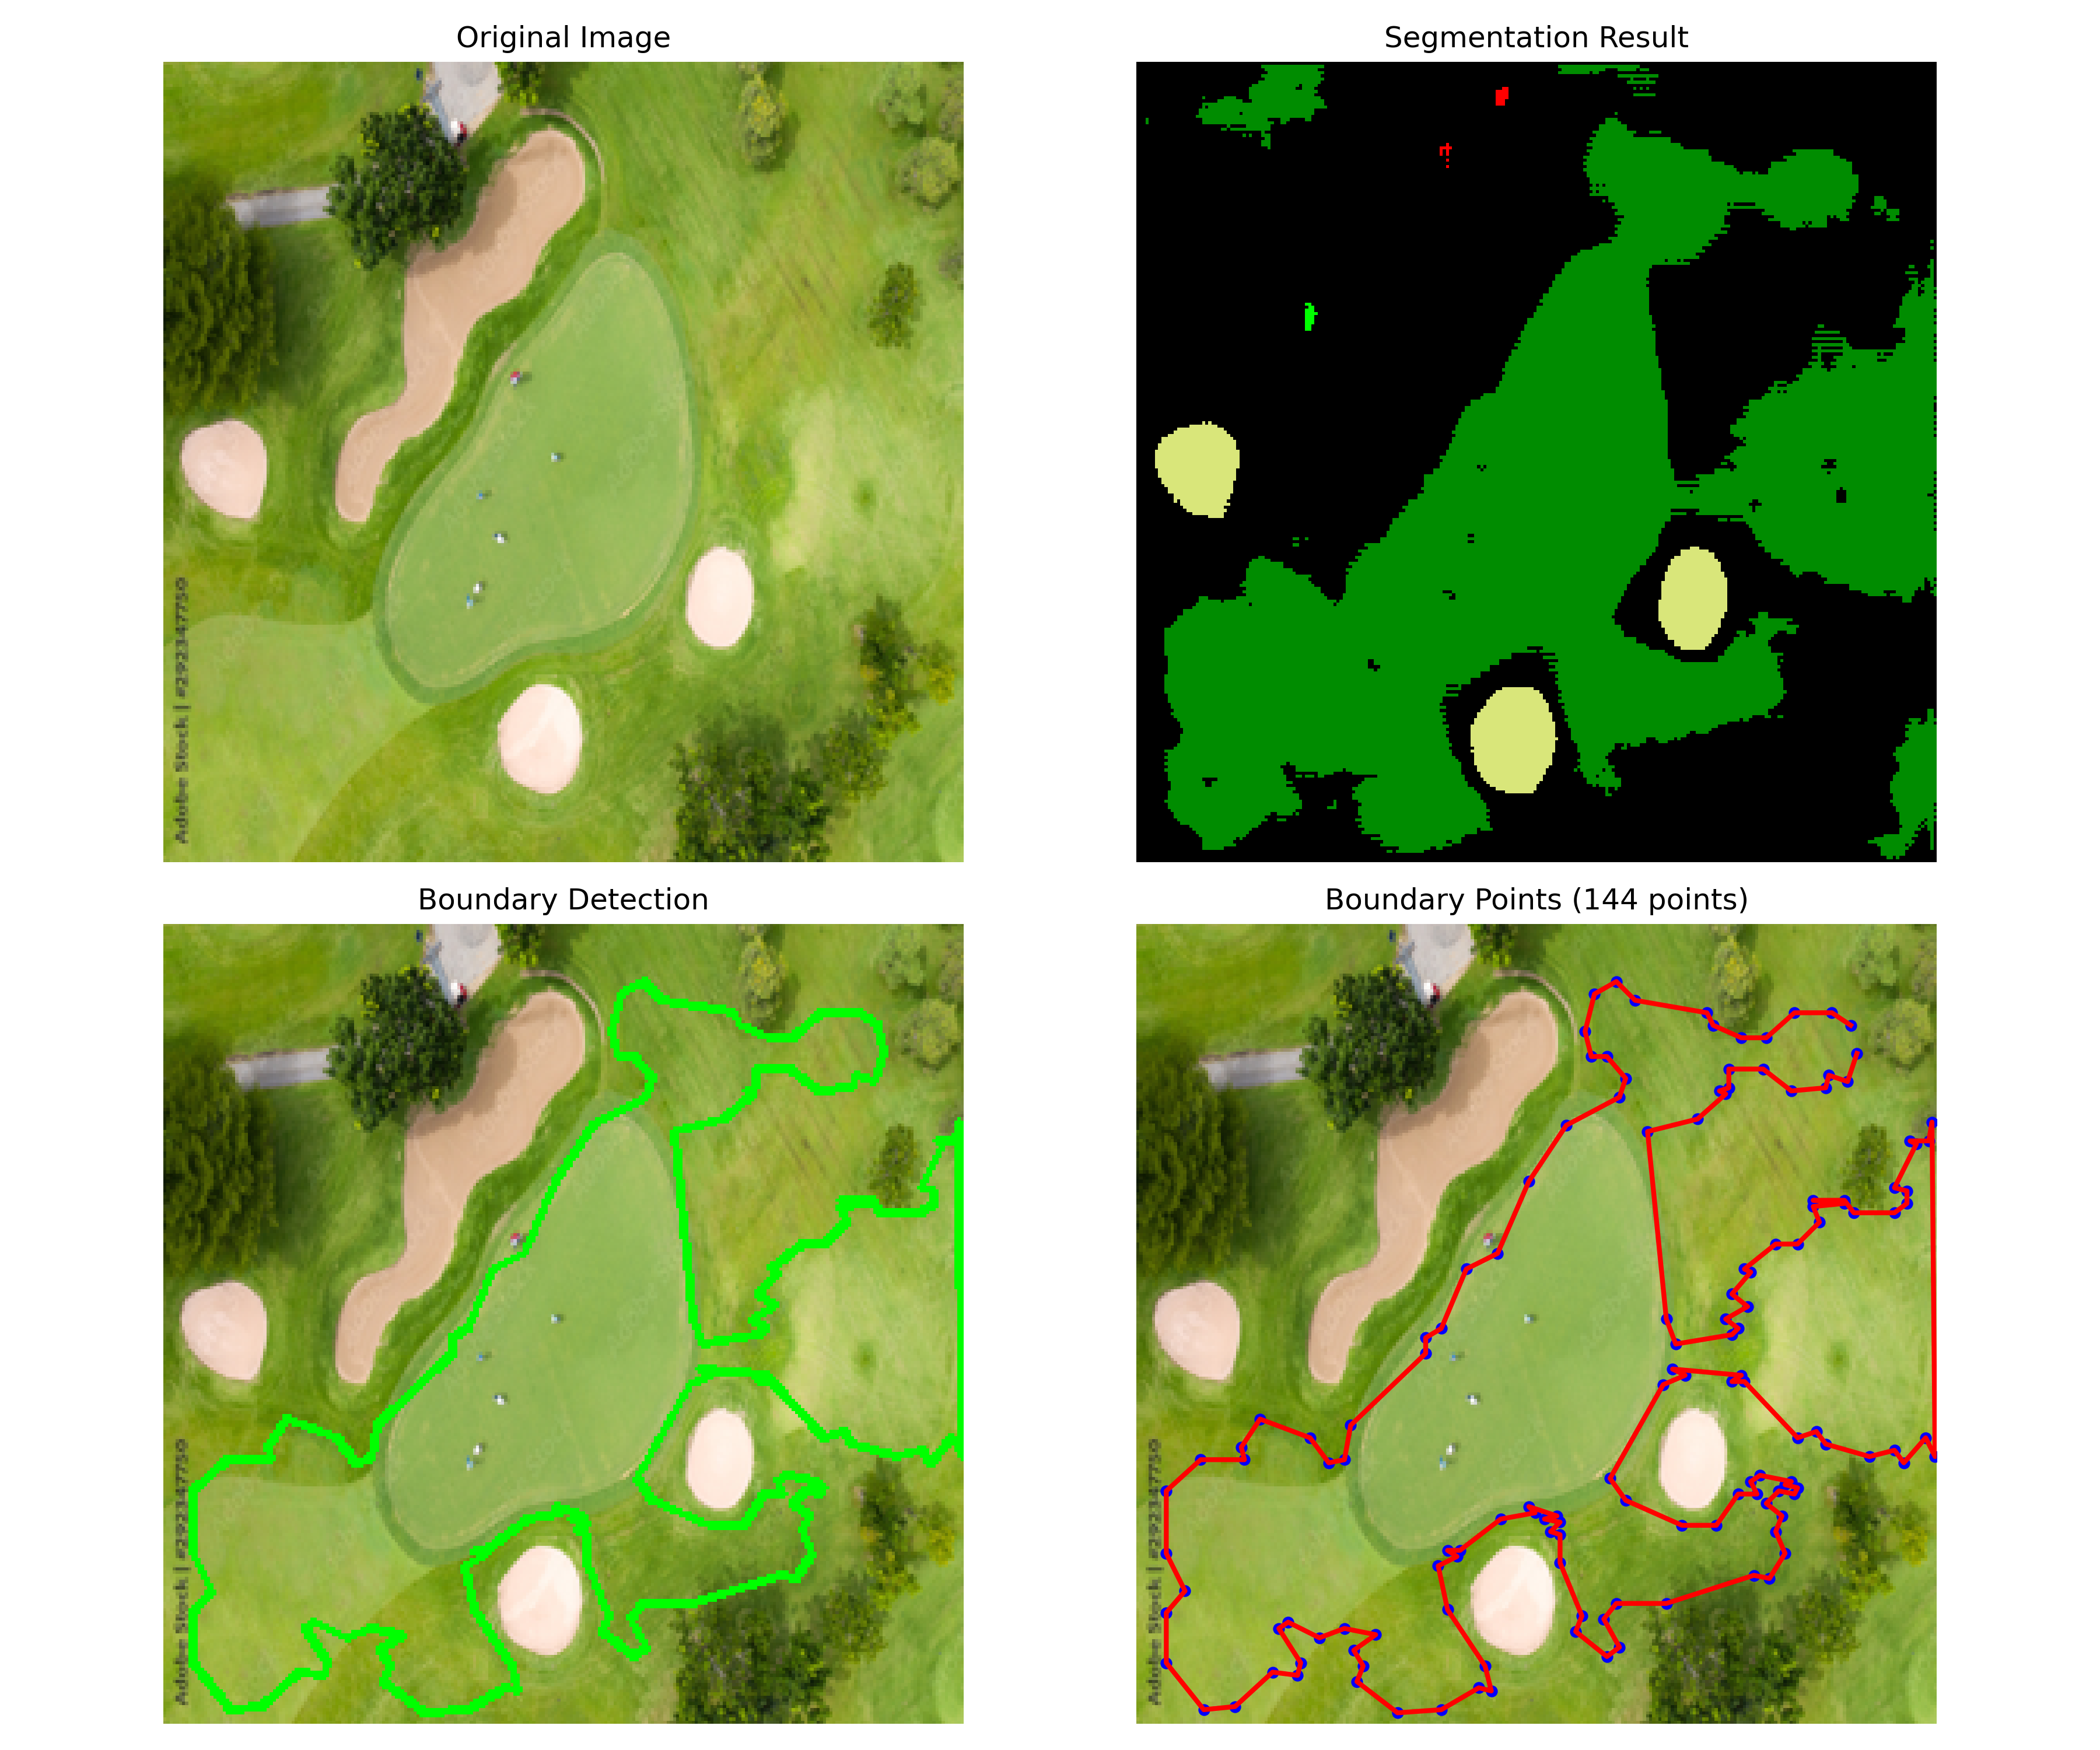
\includegraphics[width=0.7\textwidth]{./images/AdobeGolf_visualisation.png}
	\caption{An example ouput of pytorch model trained on the Danish Golf Course data set}
	\label{am:AGDanish}
\end{figure}

\begin{figure}[h!]
	\centering
	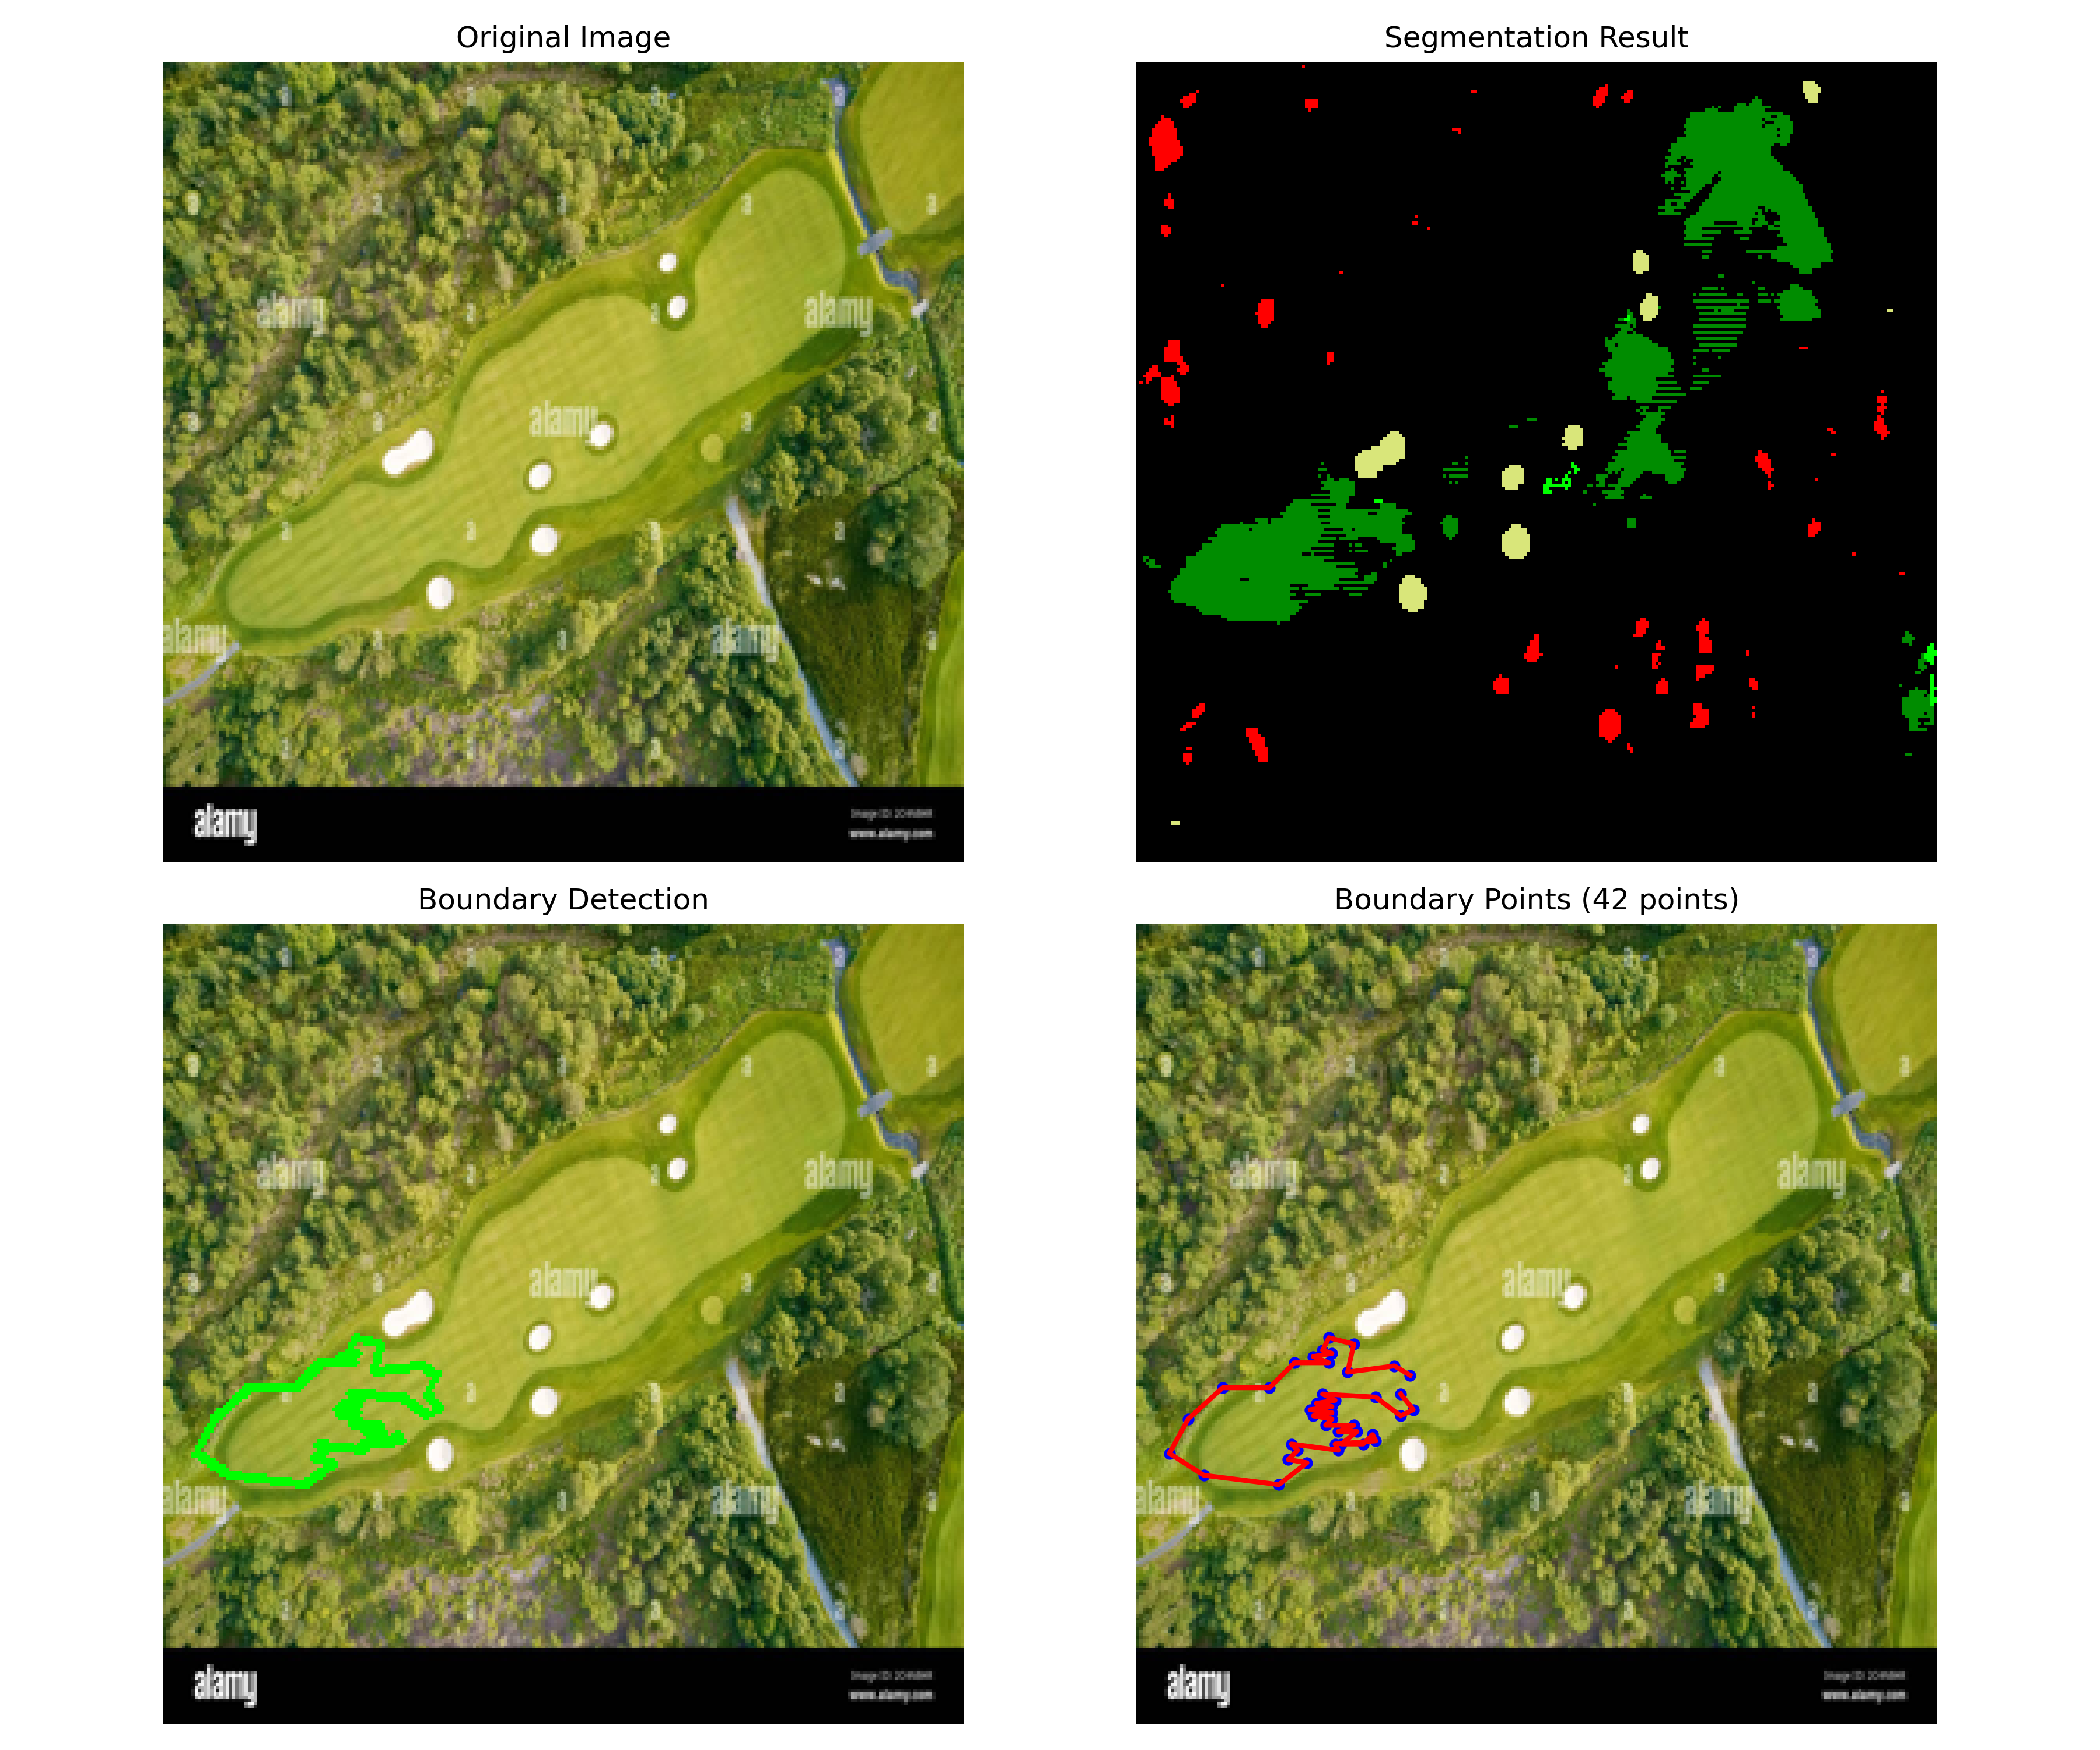
\includegraphics[width=0.6\textwidth]{./images/overheadGolfCourse_visualisation.png}
	\caption{An example ouput of pytorch model trained on the Danish Golf Course data set}
	\label{am:ohGCDanish}
\end{figure}

\begin{figure}[h!]
	\centering
	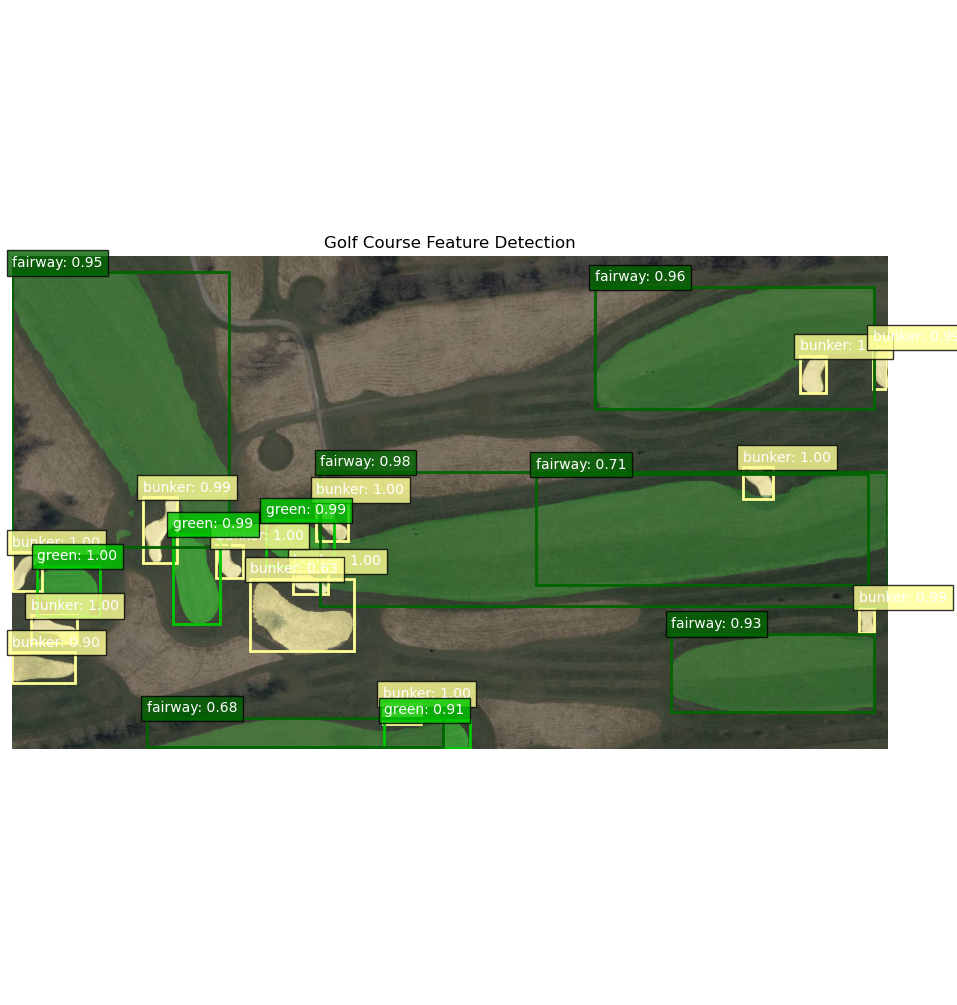
\includegraphics[width=0.6\textwidth]{./images/AENoRoughDemoTraining.png}
	\caption{Output of model trained on ~30 inputs with uncertainty at 0.7 and class weighting}
	\label{am:AENoRoughDemoTraining}
\end{figure}


\begin{figure}[h!]
	\centering
	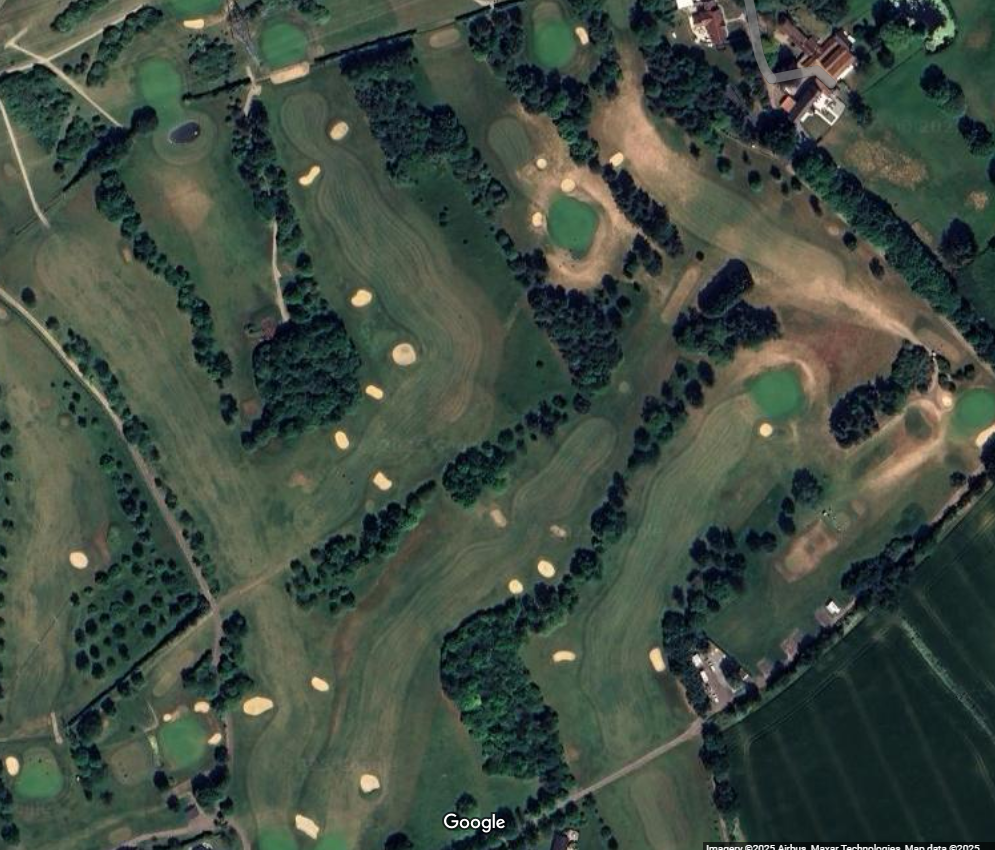
\includegraphics[width=0.5\textwidth]{./images/AEEnglishCoursePlain.png}
	\caption{Output of model trained on ~30 inputs with uncertainty at 0.7 and class weighting}
	\label{am:AEEnglishCoursePlain}
\end{figure}


\begin{figure}[h!]
	\centering
	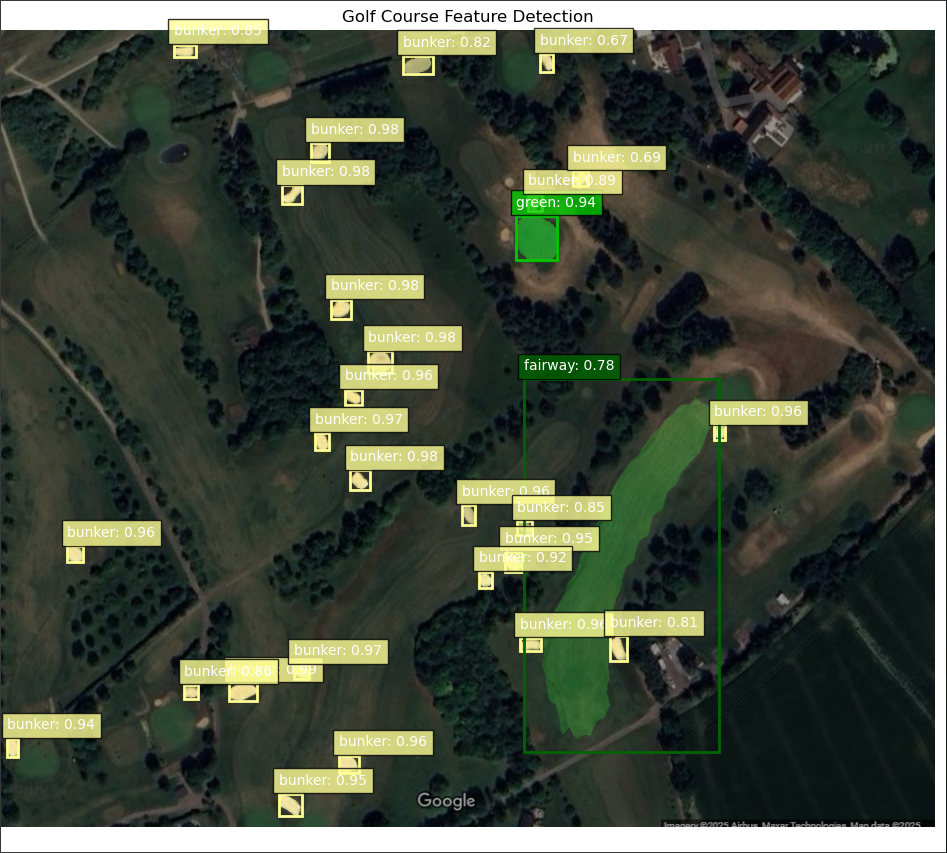
\includegraphics[width=0.7\textwidth]{./images/AEEnglishCourseResult.png}
	\caption{Output of model trained on ~30 inputs with uncertainty at 0.7 and class weighting}
	\label{am:AEEnglishCourseResult}
\end{figure}



\clearpage
\section{Performance and Evaluation}
\subsection{Mapping}


\begin{figure}[h!]
	\centering
	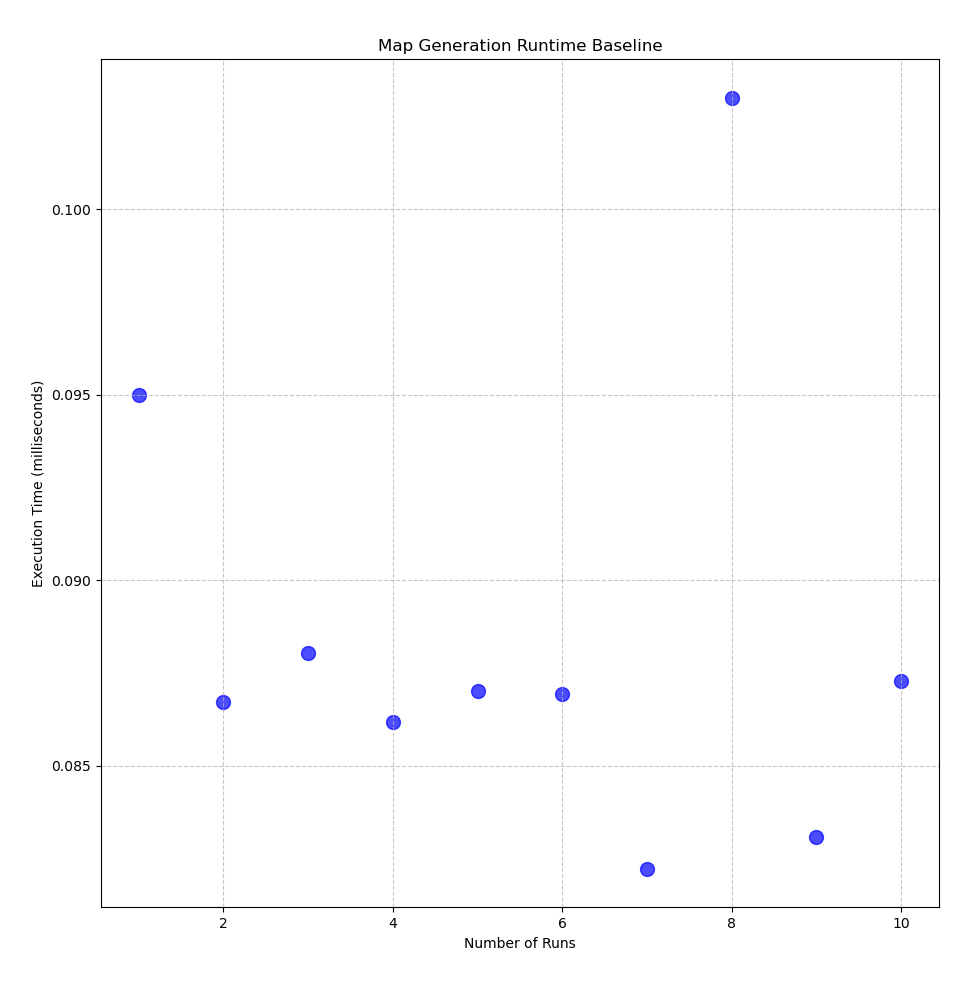
\includegraphics[width=0.45\textwidth]{./images/mapGenBaselineRT.png}
	\caption{Runtime of the map generation algorithm with 10 points, 400 range, 0 holes}
	\label{PE:mg:baselineRT}
\end{figure}


\begin{figure}[h!]
	\centering
	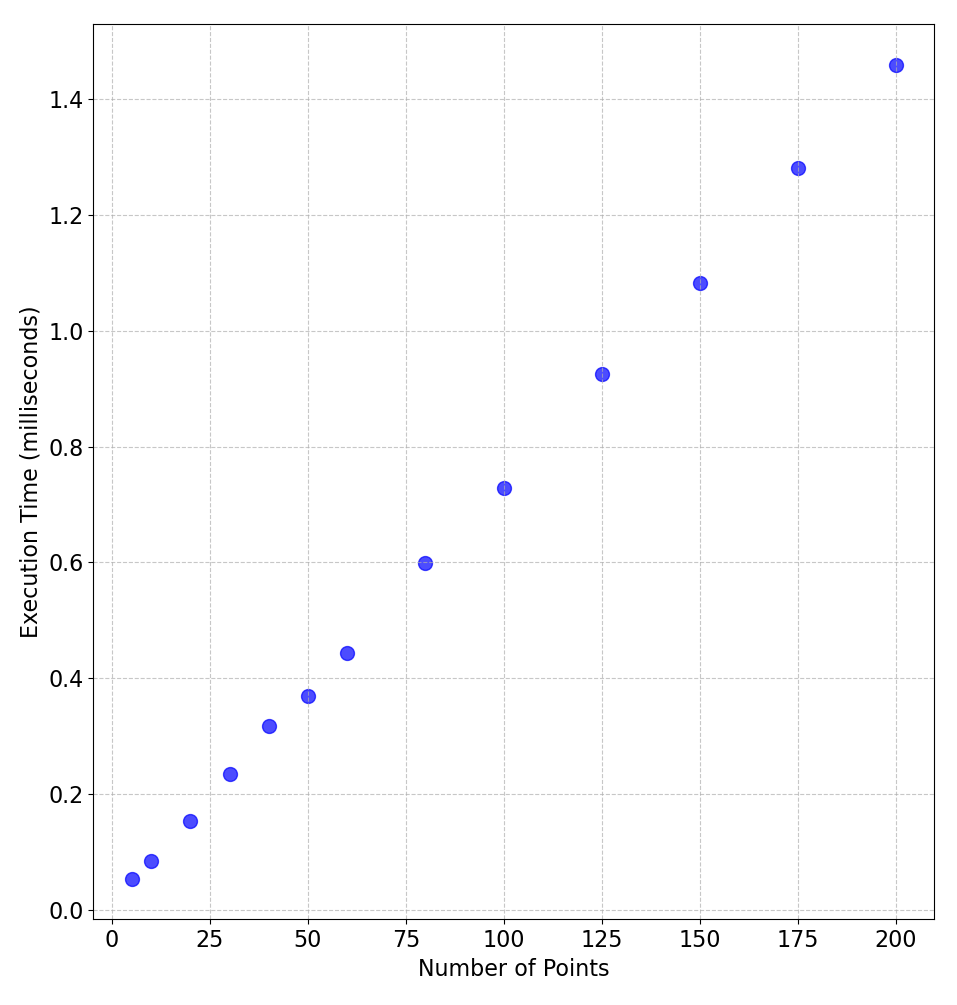
\includegraphics[width=0.45\textwidth]{./images/mapGenPointsRT.png}
	\caption{Runtime of the map generation algorithm with variable points, 400 range, 0 holes}
	\label{PE:mg:points}
\end{figure}


\begin{figure}[h!]
	\centering
	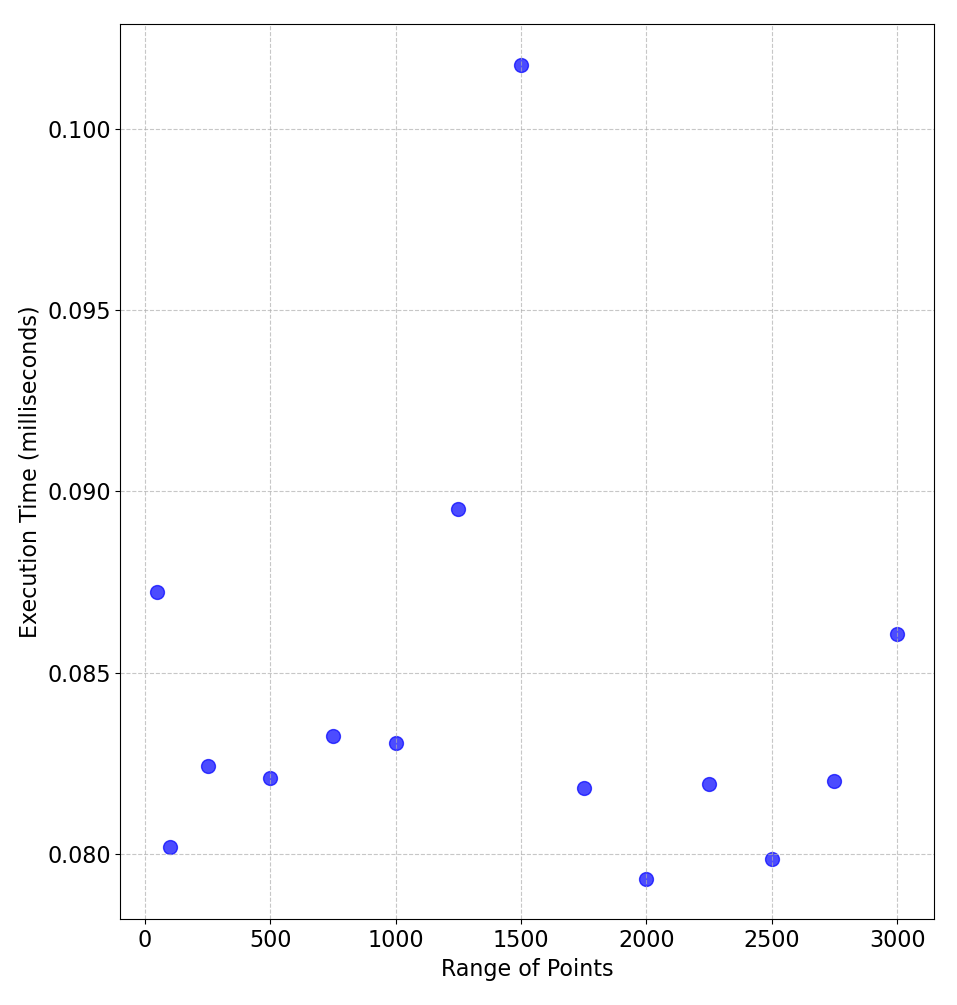
\includegraphics[width=0.5\textwidth]{./images/mapGenRangeRT.png}
	\caption{Runtime of the map generation algorithm with 10 points, variable range, 0 holes}

	\label{PE:mg:range}
\end{figure}

\begin{figure}[h!]
	\centering
	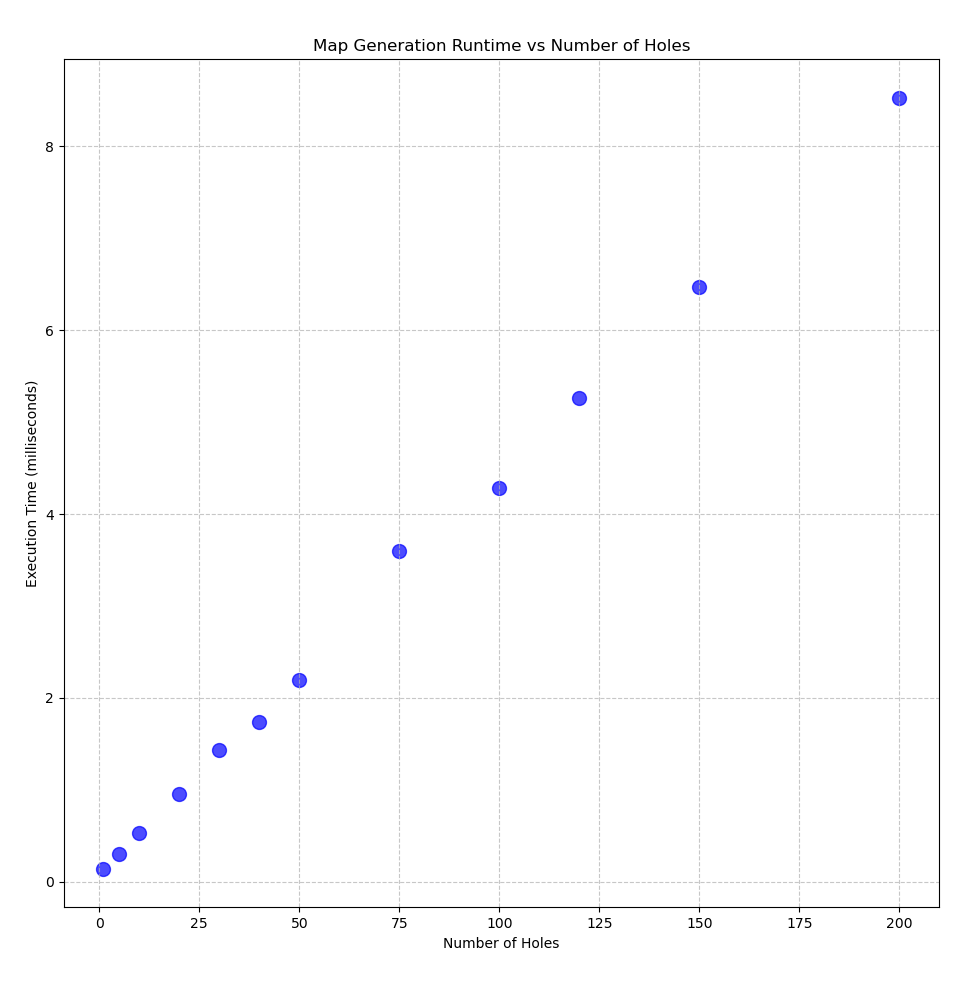
\includegraphics[width=0.5\textwidth]{./images/mapGenHolesRT.png}
	\caption{Runtime of the map generation algorithm with 10 points, 400 range, variable holes}
	\label{PE:mg:holes}
\end{figure}

\begin{figure}[h!]
	\centering
	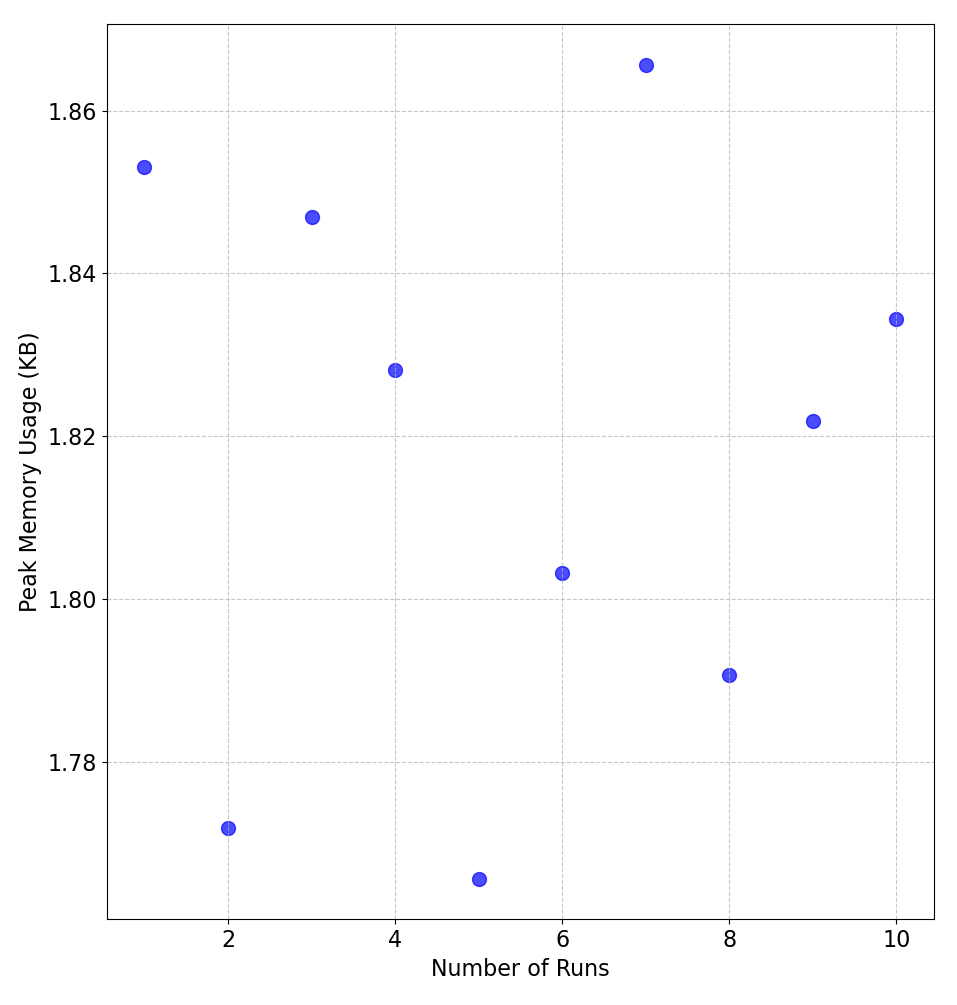
\includegraphics[width=0.5\textwidth]{./images/mapGenBaselineMem.png}
	\caption{Memory usage of map generation algorith with 10 points, 400 range, 0 holes}
	\label{PE:mg:memBaseline}
\end{figure}

\begin{figure}[h!]
	\centering
	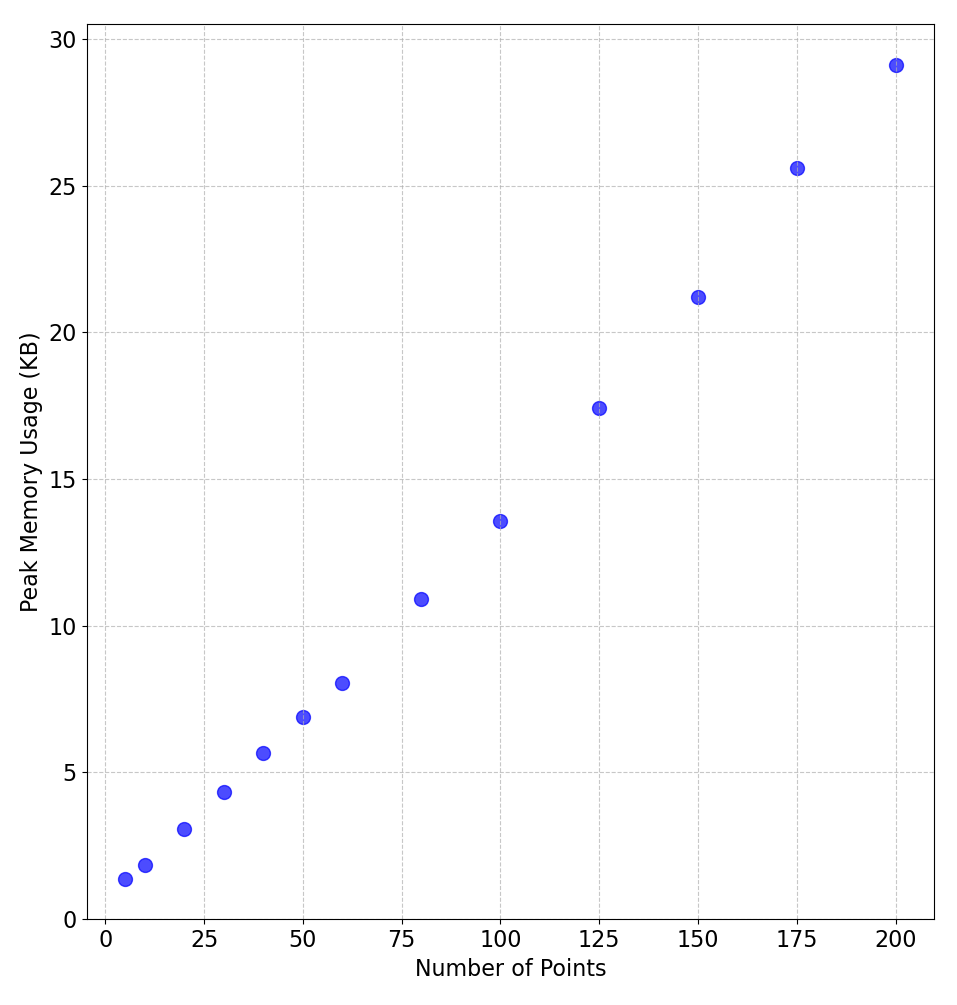
\includegraphics[width=0.5\textwidth]{./images/mapGenPointsMem.png}
	\caption{Memory usage of map generation algorith with variable points, 400 range, 0 holes}
	\label{PE:mg:memPoints}
\end{figure}

\begin{figure}[h!]
	\centering
	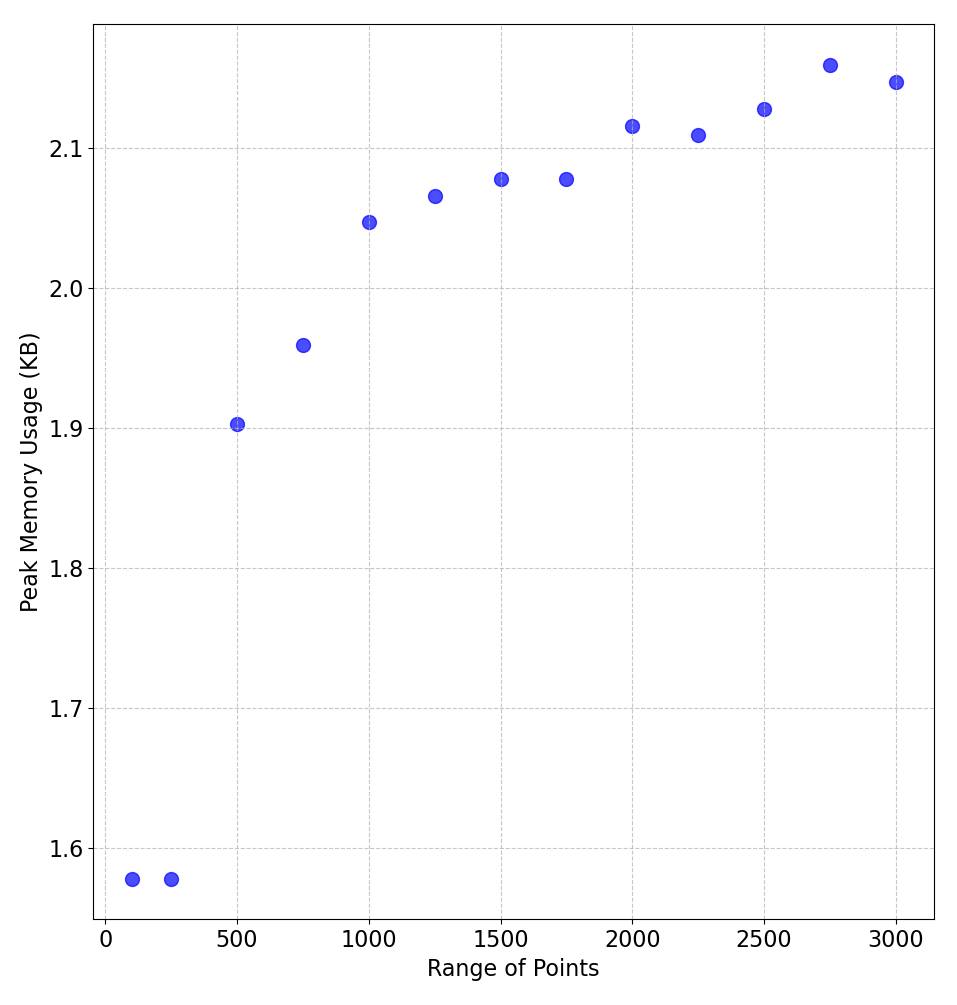
\includegraphics[width=0.5\textwidth]{./images/mapGenRangeMem.png}
	\caption{Memory usage of map generation algorith with 10 points, variable range, 0 holes}
	\label{PE:mg:memRange}
\end{figure}

\begin{figure}[h!]
	\centering
	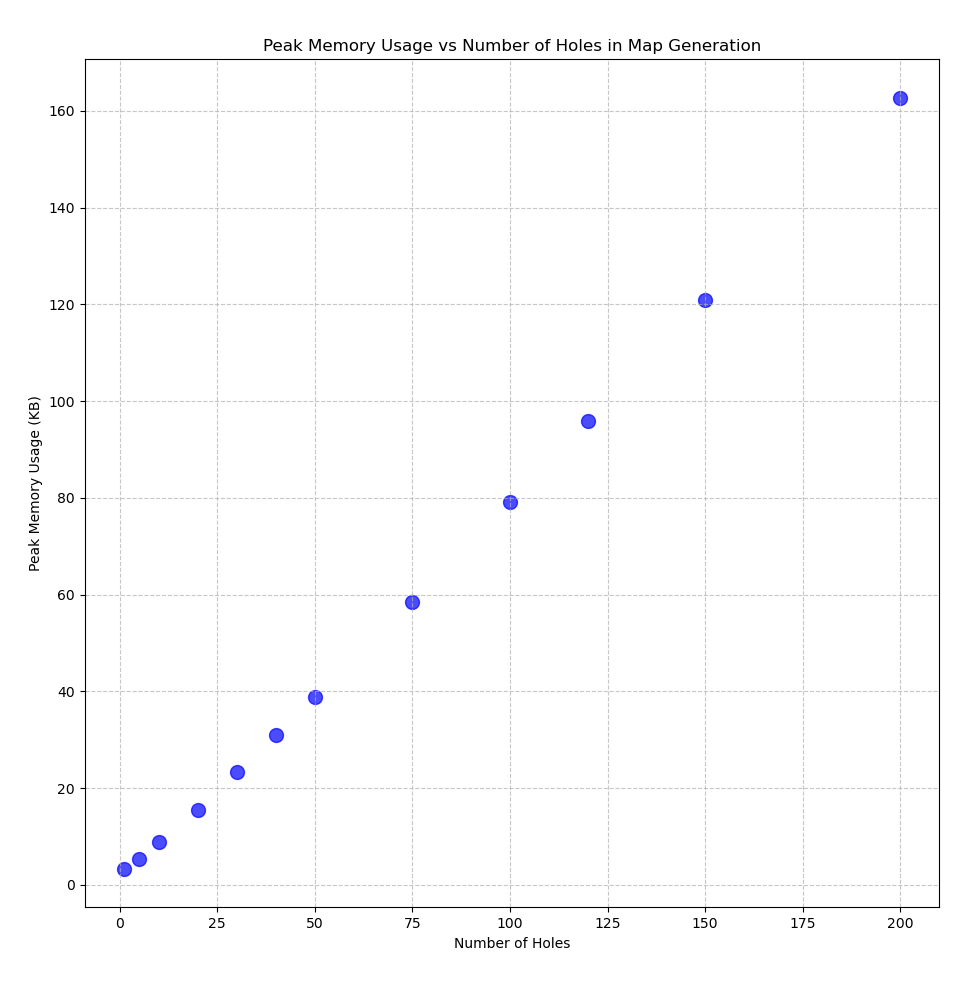
\includegraphics[width=0.5\textwidth]{./images/mapGenHolesMem.png}
	\caption{Memory usage of map generation algorith with 10 points, 400 range, variable holes}
	\label{PE:mg:memHoles}
\end{figure}


\clearpage
\subsection{Pathing}
\begin{figure}[h!]
	\centering
	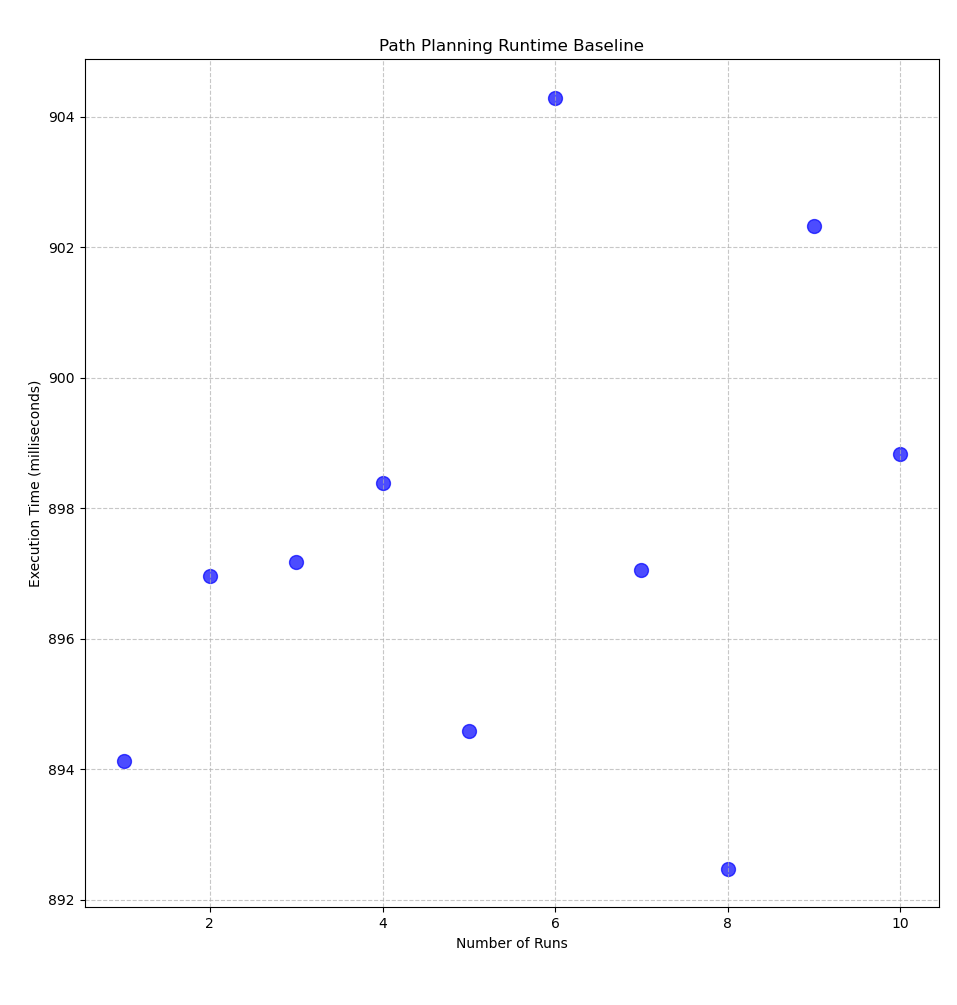
\includegraphics[width=0.45\textwidth]{./images/pathingBaseLineRT.png}
	\caption{Runtime of path planning system with $10^3m^2$ area, 6 corners, accurate robot size, constant headland, brute force swath gen, Reeds-Shepp pathing and shortest route planning}
	\label{PE:p:BaselineRT}
\end{figure}


\begin{figure}[h!]
	\centering
	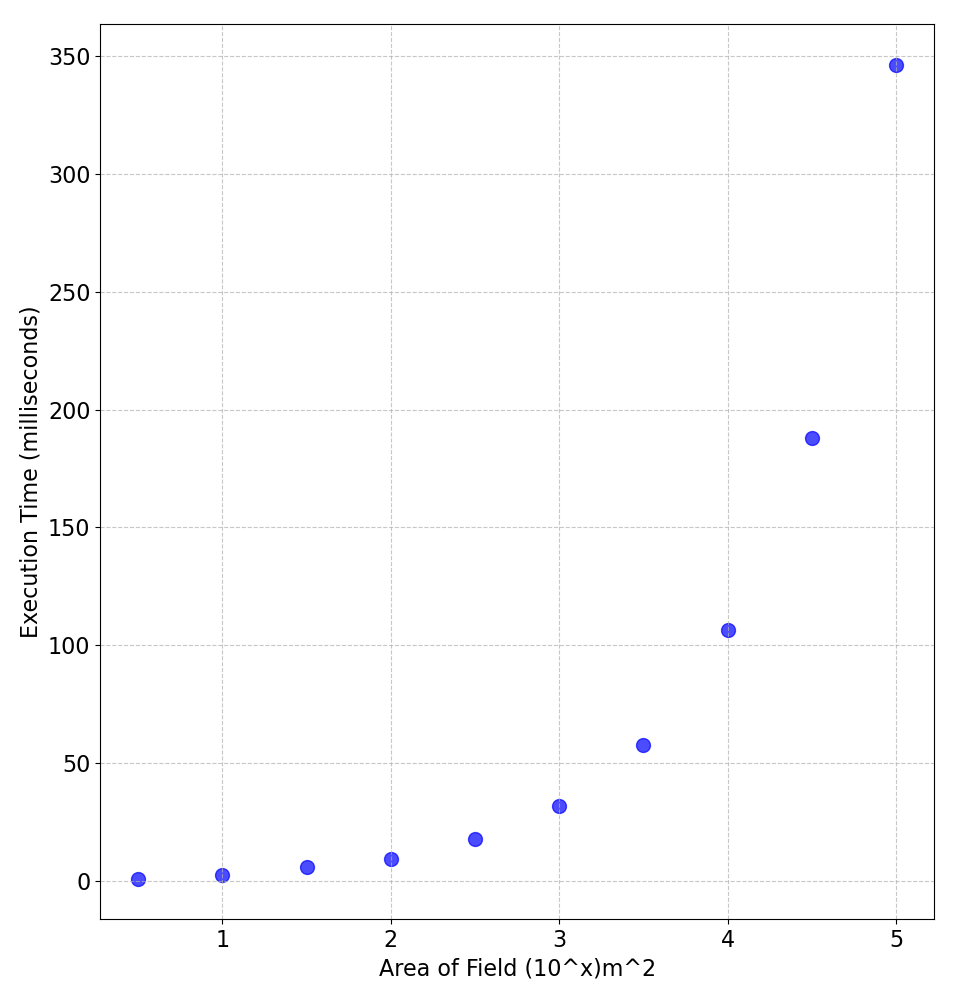
\includegraphics[width=0.45\textwidth]{./images/pathingSizeRt.png}
	\caption{Runtime of path planning system with $10^3m^2$ area, 6 corners, accurate robot size, constant headland, brute force swath gen, Reeds-Shepp pathing and shortest route planning}
	\label{PE:p:SizeRT}
\end{figure}


\begin{figure}[h!]
	\centering
	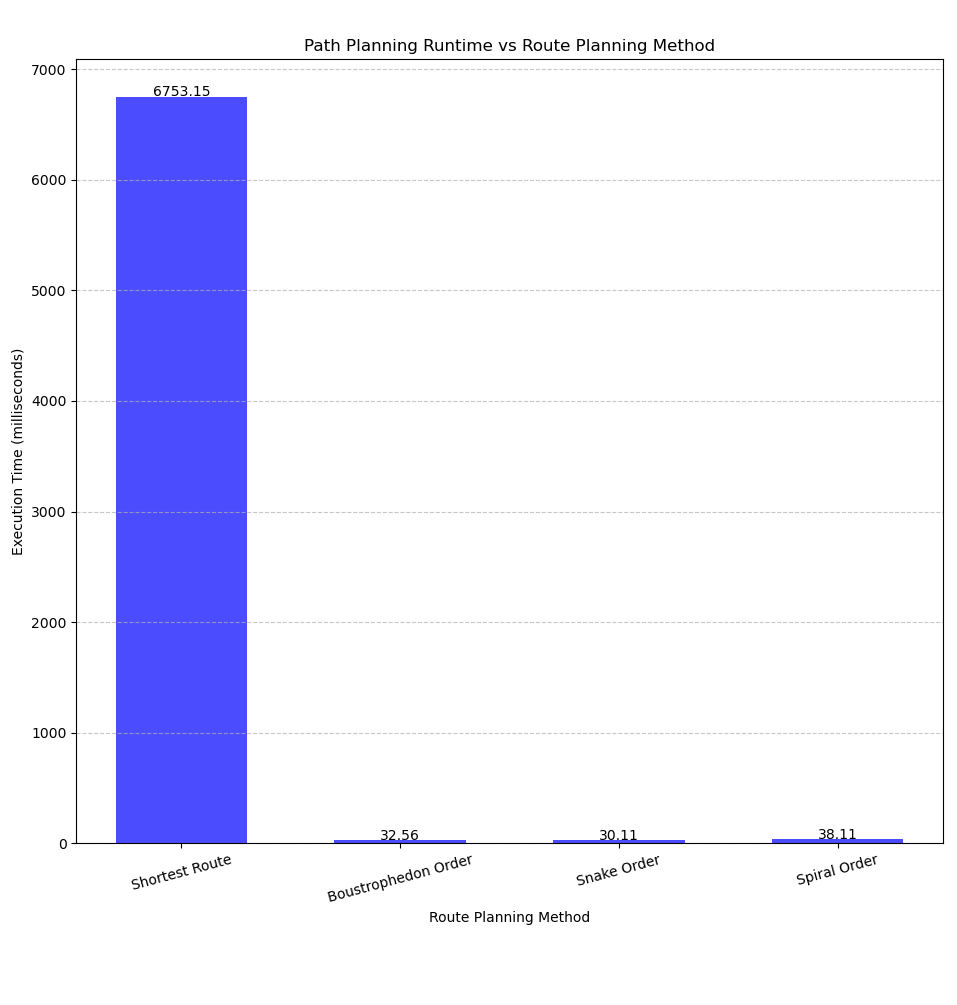
\includegraphics[width=0.5\textwidth]{./images/pathingRoutePlanningRT.png}
	\caption{Runtime of path planning system with $10^3m^2$ area, 6 corners, accurate robot size, constant headland, brute force swath gen, variable pathing and shortest route planning}
	\label{PE:p:RoutePlanningRT}
\end{figure}


\begin{figure}[h!]
	\centering
	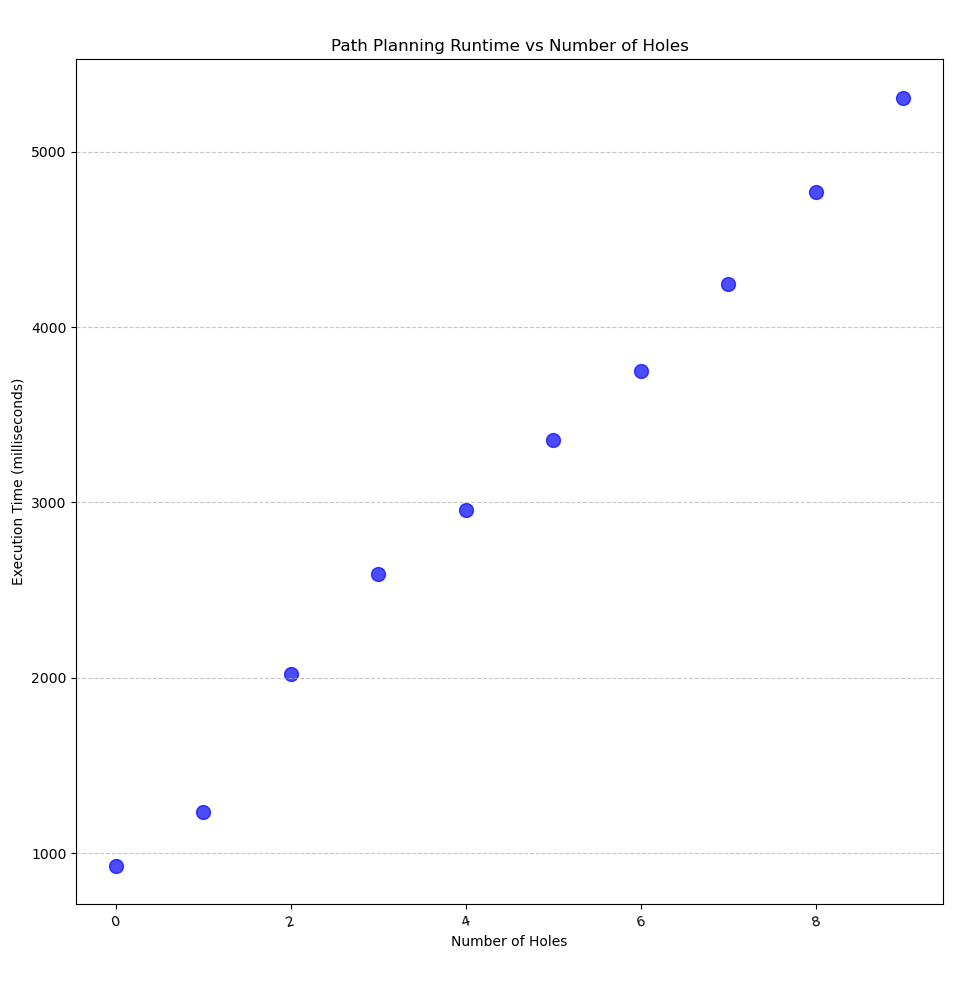
\includegraphics[width=0.5\textwidth]{./images/pathingHolesRT.png}
	\caption{Runtime of path planning system with $10^3m^2$ area, 6 corners, accurate robot size, constant headland, brute force swath gen, Reeds-Shepp pathing, shortest route planning and variable holes}
	\label{PE:p:HolesRT}
\end{figure}


\begin{figure}[h!]
	\centering
	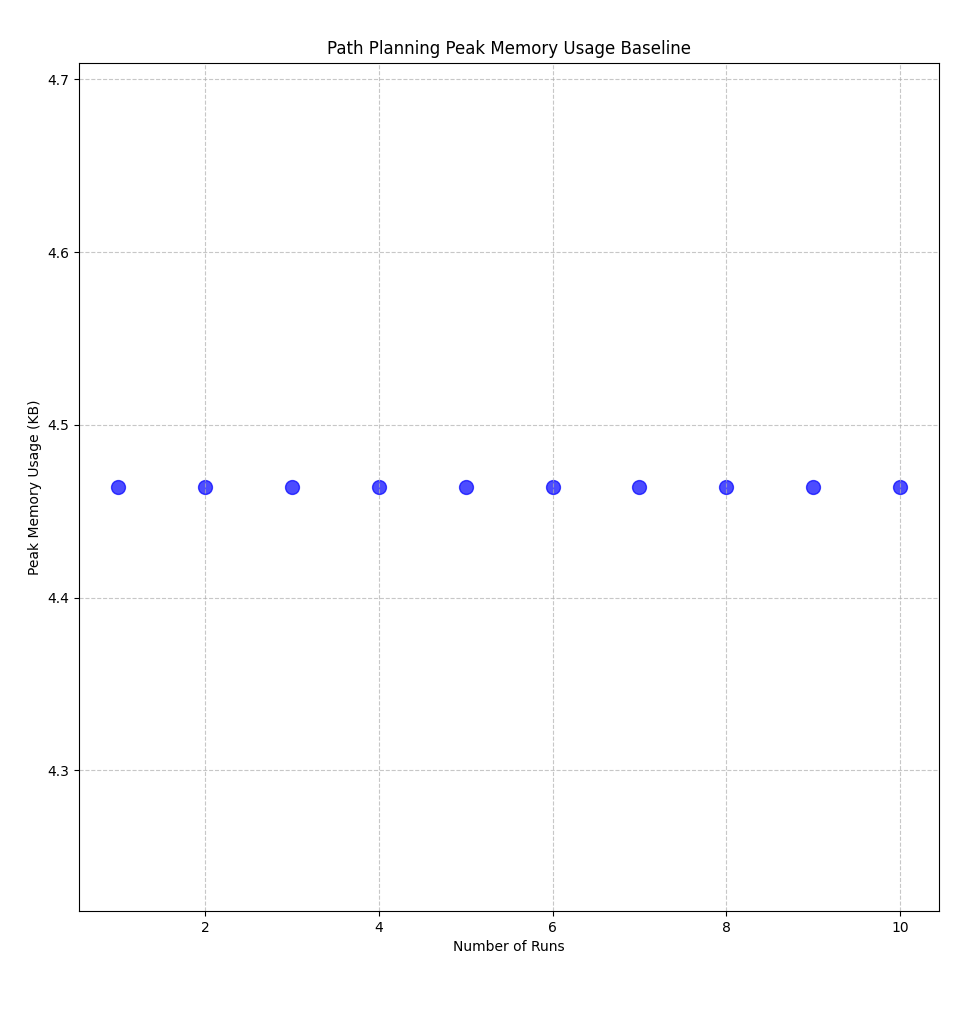
\includegraphics[width=0.8\textwidth]{./images/pathingBaseLineMem.png}
	\caption{Memory Usage of path planning system with $10^3m^2$ area, 6 corners, accurate robot size, constant headland, brute force swath gen, Reeds-Shepp pathing and shortest route planning}
	\label{PE:p:BaselineMem}
\end{figure}


\begin{figure}[h!]
	\centering
	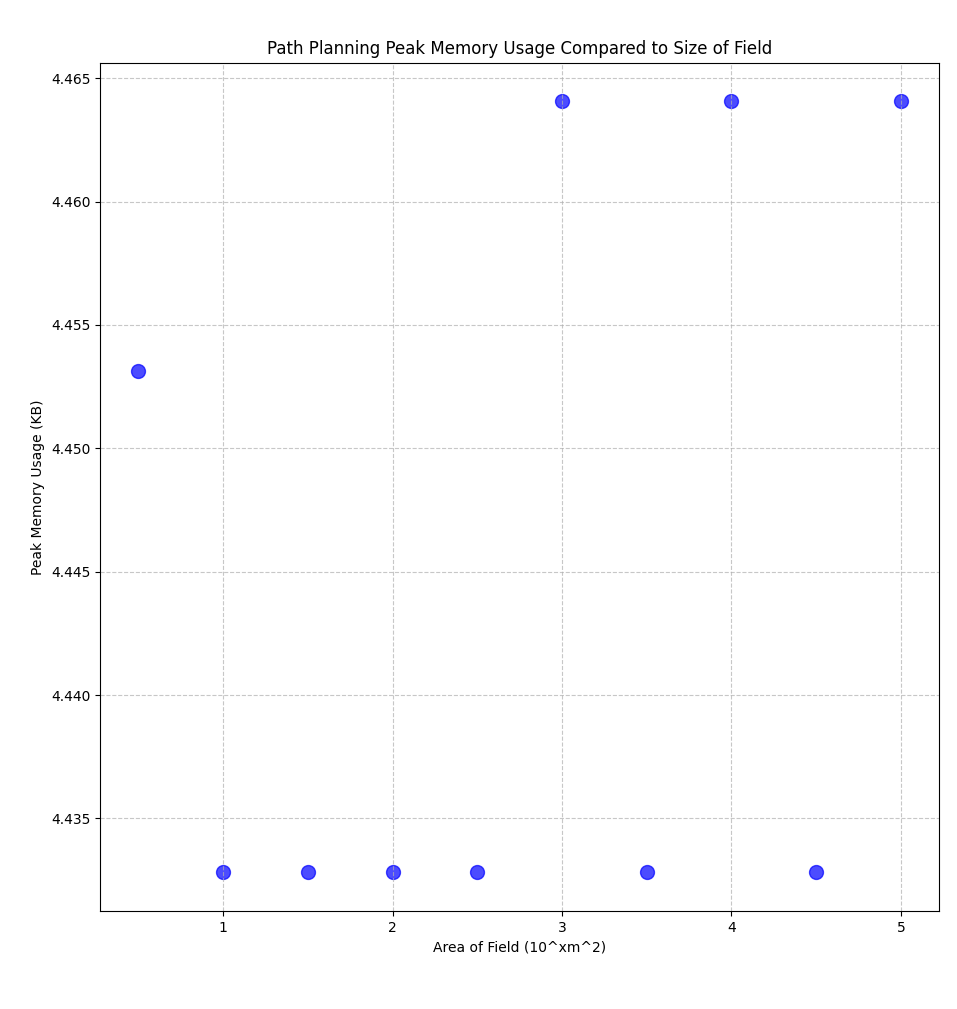
\includegraphics[width=0.5\textwidth]{./images/pathingSizeMem.png}
	\caption{Memory Usage of path planning system with variable area, 6 corners, accurate robot size, constant headland, brute force swath gen, Reeds-Shepp pathing and shortest route planning}
	\label{PE:p:SizeMem}
\end{figure}


\begin{figure}[h!]
	\centering
	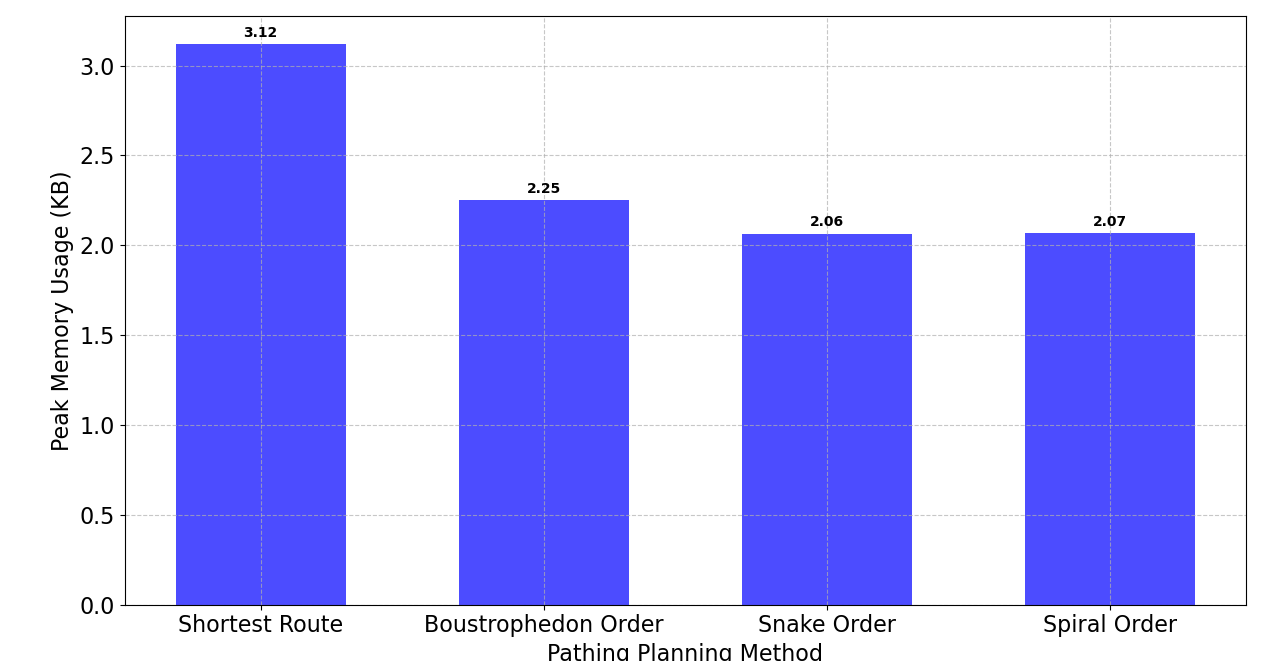
\includegraphics[width=0.9\textwidth]{./images/pathingRoutePlanningMem.png}
	\caption{Memory Usage of path planning system with $10^3m^2$ area, 6 corners, accurate robot size, constant headland, brute force swath gen, variable pathing and shortest route planning}
	\label{PE:p:RoutePlanningMem}
\end{figure}


\begin{figure}[h!]
	\centering
	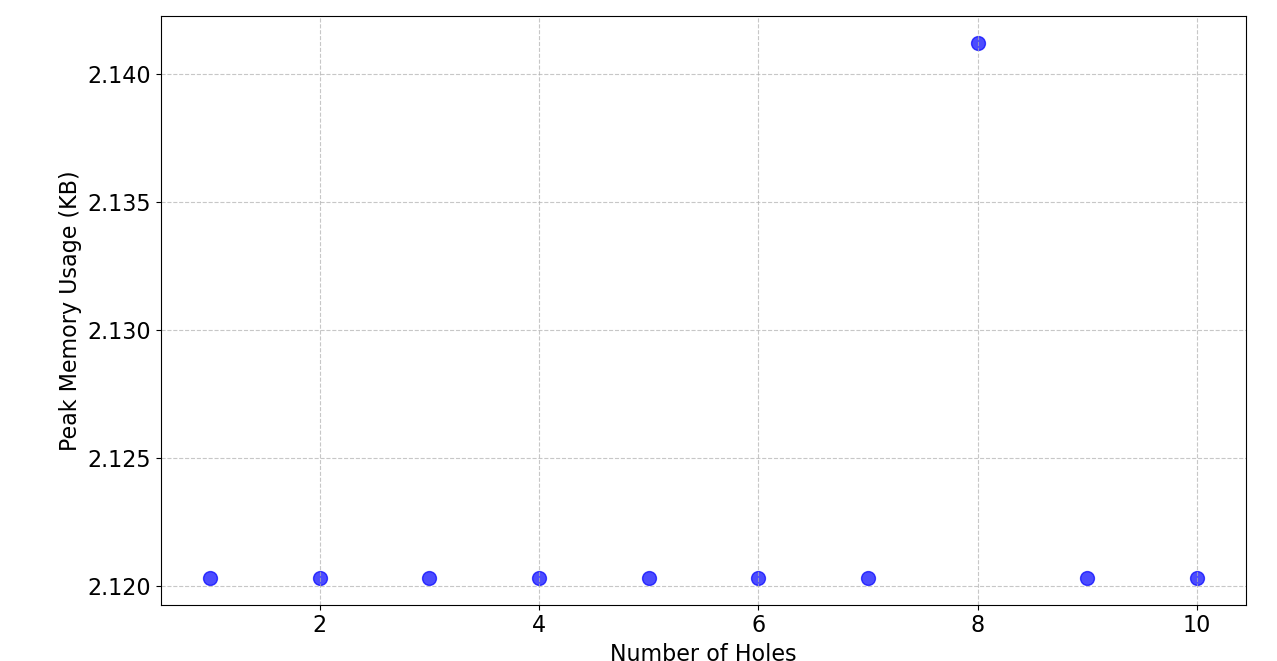
\includegraphics[width=0.5\textwidth]{./images/pathingHolesMem.png}
	\caption{Memory Usage of path planning system with $10^3m^2$ area, 6 corners, accurate robot size, constant headland, brute force swath gen, Reeds-Shepp pathing, shortest route planning and variable number of holes}
	\label{PE:p:HolesMem}
\end{figure}


\clearpage
\subsubsection{Aerial Mapping}
%
% \begin{figure}[h!]
% 	\centering
% 	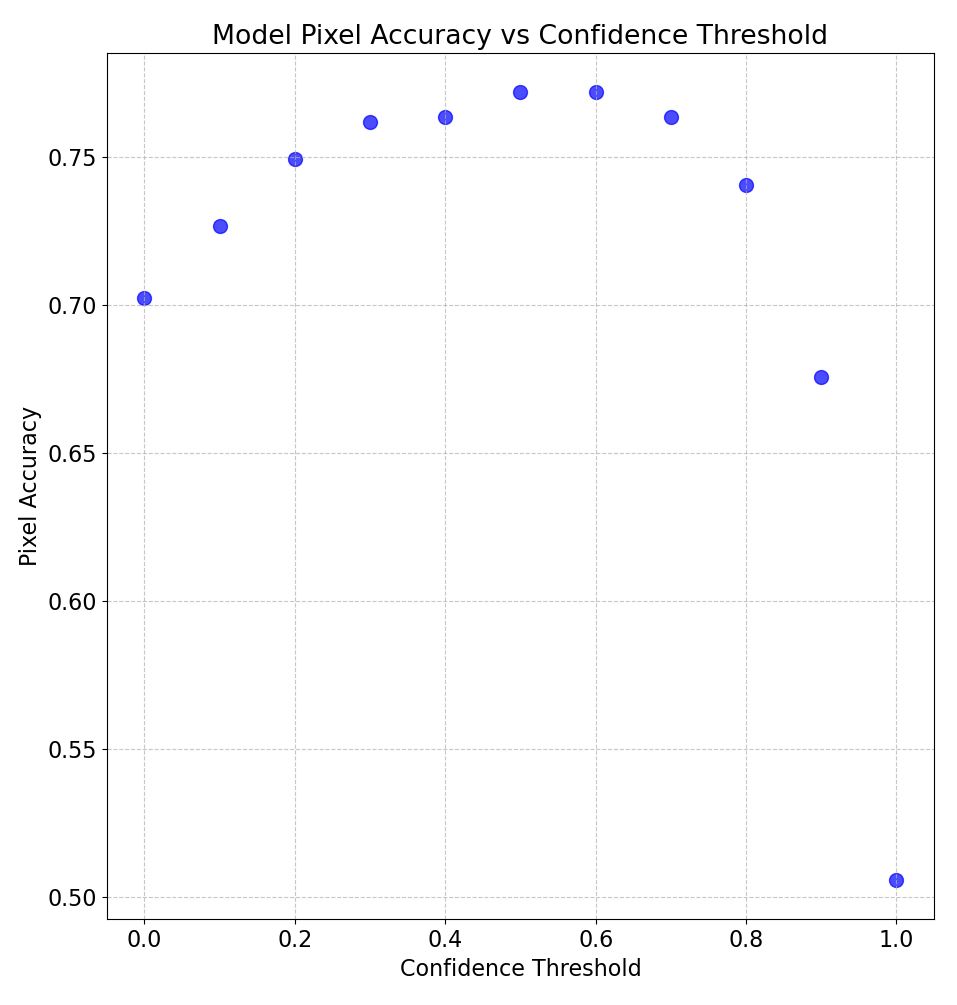
\includegraphics[width=0.5\textwidth]{./images/AEConfidenceThreshold.png}
% 	\caption{Pixel accuracy vs confidence threshold of maskRCNN model}
% 	\label{AE:ConfidenceThreshold}
% \end{figure}
%
% \begin{figure}[h!]
% 	\centering
% 	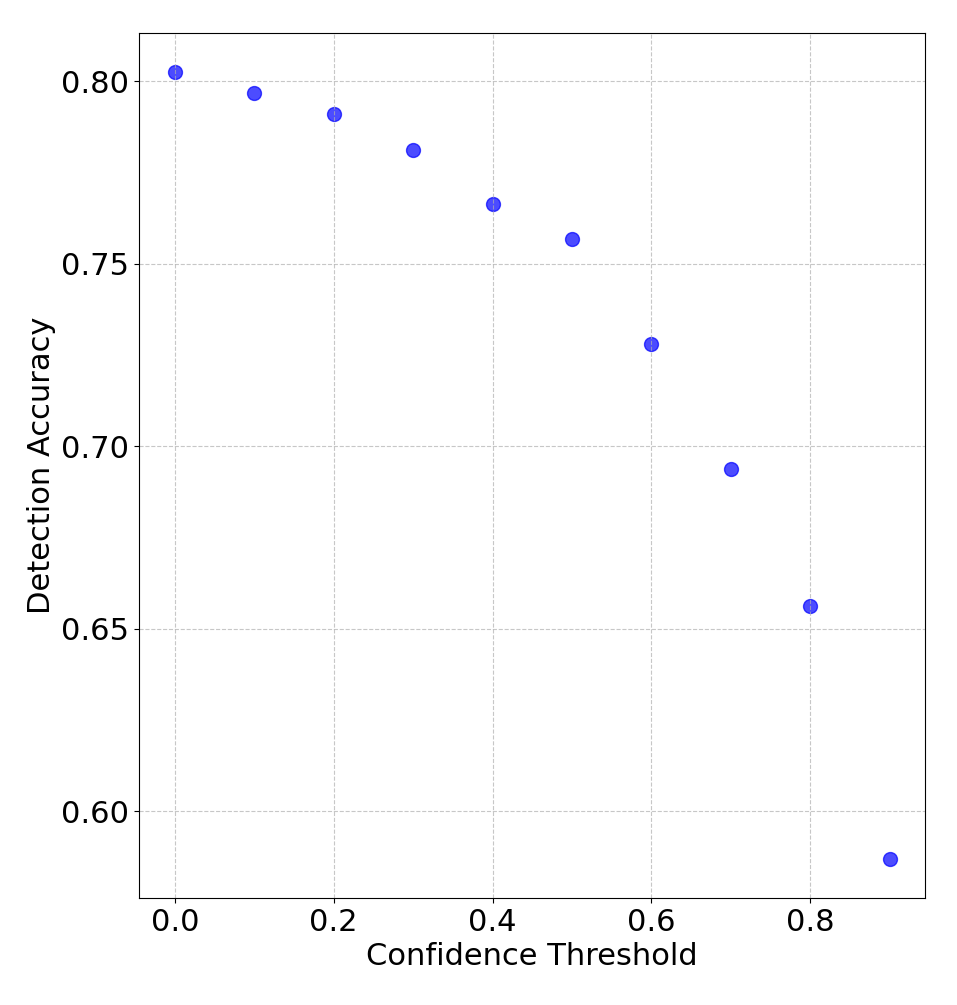
\includegraphics[width=0.5\textwidth]{./images/AEConfidenceThresholdDetect.png}
% 	\caption{Detection accuracy vs confidence threshold of maskRCNN model}
% 	\label{AE:ConfidenceThresholdDetect}
% \end{figure}
%
% \begin{figure}[h!]
% 	\centering
% 	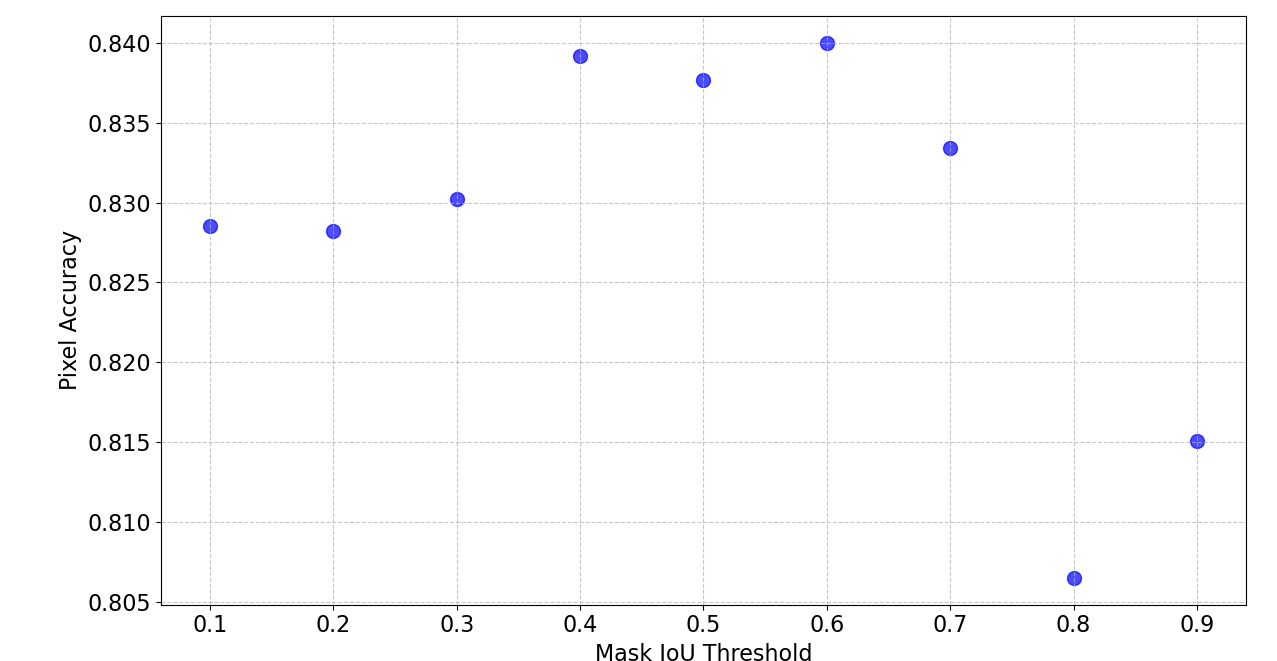
\includegraphics[width=0.9\textwidth]{./images/AEIOUThresholdPixel.png}
% 	\caption{Pixel accuracy vs intersection over union of maskRCNN model}
% 	\label{AE:IOUThreshold}
% \end{figure}
%
% \begin{figure}[h!]
% 	\centering
% 	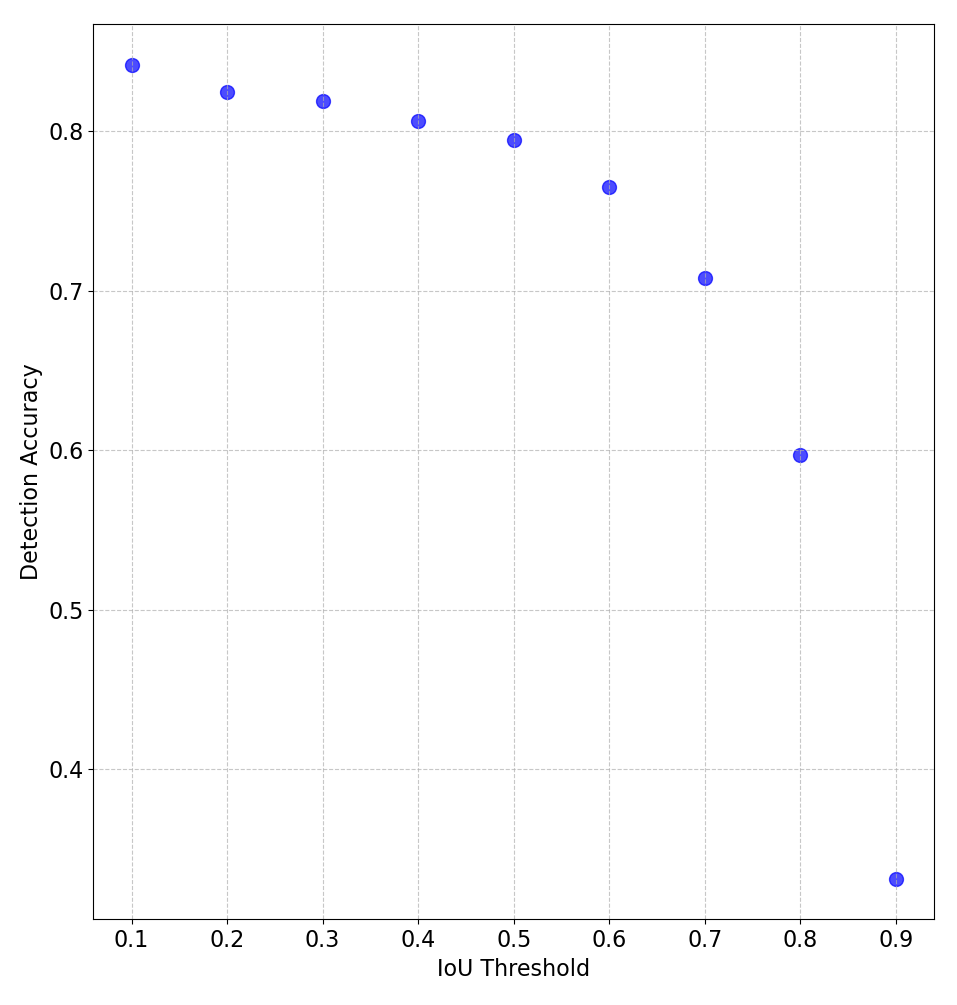
\includegraphics[width=0.5\textwidth]{./images/AEIOUThresholdDetect.png}
% 	\caption{Detection accuracy vs intersection over union of maskRCNN model}
% 	\label{AE:IOUThresholdDetect}
% \end{figure}
%
%
%
%
%



\begin{figure}[h!]
	\centering
	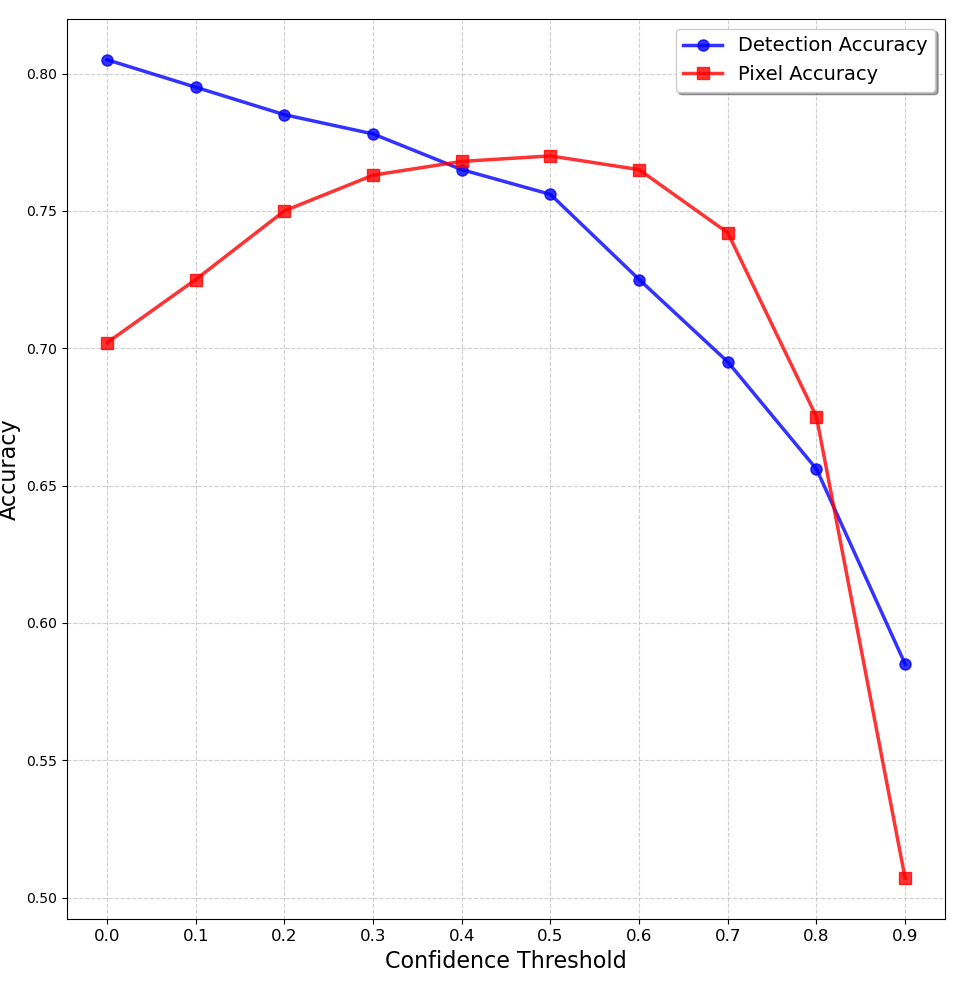
\includegraphics[width=0.5\textwidth]{./images/AEConfidenceCombined.png}
	\caption{Pixel and detection accuracy vs confidence threshold of maskRCNN model}
	\label{AE:Confidence}
\end{figure}

\begin{figure}[h!]
	\centering
	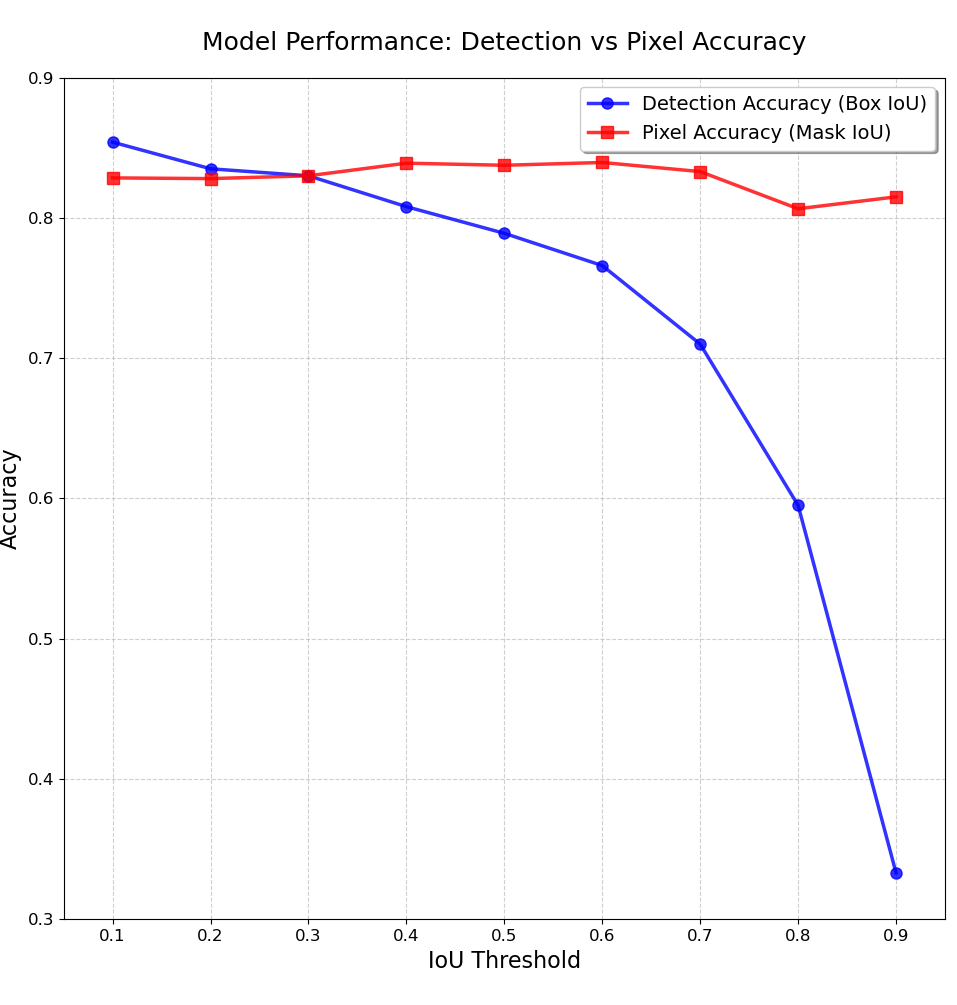
\includegraphics[width=0.5\textwidth]{./images/AEIOUCombined.png}
	\caption{Pixel accuracy vs intersection over union threshold of maskRCNN model}
	\label{AE:IOU}
\end{figure}


\end{document}
